% Template for PLoS
% Version 3.6 Aug 2022
%
% % % % % % % % % % % % % % % % % % % % % %
%
% -- IMPORTANT NOTE
%
% This template contains comments intended
% to minimize problems and delays during our production
% process. Please follow the template instructions
% whenever possible.
%
% % % % % % % % % % % % % % % % % % % % % % %
%
% Once your paper is accepted for publication,
% PLEASE REMOVE ALL TRACKED CHANGES in this file
% and leave only the final text of your manuscript.
% PLOS recommends the use of latexdiff to track changes during review, as this will help to maintain a clean tex file.
% Visit https://www.ctan.org/pkg/latexdiff?lang=en for info or contact us at latex@plos.org.
%
%
% There are no restrictions on package use within the LaTeX files except that no packages listed in the template may be deleted.
%
% Please do not include colors or graphics in the text.
%
% The manuscript LaTeX source should be contained within a single file (do not use \input, \externaldocument, or similar commands).
%
% % % % % % % % % % % % % % % % % % % % % % %
%
% -- FIGURES AND TABLES
%
% Please include tables/figure captions directly after the paragraph where they are first cited in the text.
%
% DO NOT INCLUDE GRAPHICS IN YOUR MANUSCRIPT
% - Figures should be uploaded separately from your manuscript file.
% - Figures generated using LaTeX should be extracted and removed from the PDF before submission.
% - Figures containing multiple panels/subfigures must be combined into one image file before submission.
% For figure citations, please use "Fig" instead of "Figure".
% See http://journals.plos.org/plosone/s/figures for PLOS figure guidelines.
%
% Tables should be cell-based and may not contain:
% - spacing/line breaks within cells to alter layout or alignment
% - do not nest tabular environments (no tabular environments within tabular environments)
% - no graphics or colored text (cell background color/shading OK)
% See http://journals.plos.org/plosone/s/tables for table guidelines.
%
% For tables that exceed the width of the text column, use the adjustwidth environment as illustrated in the example table in text below.
%
% % % % % % % % % % % % % % % % % % % % % % % %
%
% -- EQUATIONS, MATH SYMBOLS, SUBSCRIPTS, AND SUPERSCRIPTS
%
% IMPORTANT
% Below are a few tips to help format your equations and other special characters according to our specifications. For more tips to help reduce the possibility of formatting errors during conversion, please see our LaTeX guidelines at http://journals.plos.org/plosone/s/latex
%
% For inline equations, please be sure to include all portions of an equation in the math environment.  For example, x$^2$ is incorrect; this should be formatted as $x^2$ (or $\mathrm{x}^2$ if the romanized font is desired).
%
% Do not include text that is not math in the math environment. For example, CO2 should be written as CO\textsubscript{2} instead of CO$_2$.
%
% Please add line breaks to long display equations when possible in order to fit size of the column.
%
% For inline equations, please do not include punctuation (commas, etc) within the math environment unless this is part of the equation.
%
% When adding superscript or subscripts outside of brackets/braces, please group using {}.  For example, change "[U(D,E,\gamma)]^2" to "{[U(D,E,\gamma)]}^2".
%
% Do not use \cal for caligraphic font.  Instead, use \mathcal{}
%
% % % % % % % % % % % % % % % % % % % % % % % %
%
% Please contact latex@plos.org with any questions.
%
% % % % % % % % % % % % % % % % % % % % % % % %

\documentclass[10pt,letterpaper]{article}
\usepackage[top=0.85in,left=2.75in,footskip=0.75in]{geometry}

% amsmath and amssymb packages, useful for mathematical formulas and symbols
\usepackage{amsmath,amssymb}

% Use adjustwidth environment to exceed column width (see example table in text)
\usepackage{changepage}

% textcomp package and marvosym package for additional characters
\usepackage{textcomp,marvosym}

% cite package, to clean up citations in the main text. Do not remove.
\usepackage{cite}

% Use nameref to cite supporting information files (see Supporting Information section for more info)
\usepackage{nameref,hyperref}

% line numbers
\usepackage[right]{lineno}

% ligatures disabled
\usepackage[nopatch=eqnum]{microtype}
\DisableLigatures[f]{encoding = *, family = * }

% color can be used to apply background shading to table cells only
\usepackage[table]{xcolor}

% array package and thick rules for tables
\usepackage{array}

% create "+" rule type for thick vertical lines
\newcolumntype{+}{!{\vrule width 2pt}}

% create \thickcline for thick horizontal lines of variable length
\newlength\savedwidth
\newcommand\thickcline[1]{%
  \noalign{\global\savedwidth\arrayrulewidth\global\arrayrulewidth 2pt}%
  \cline{#1}%
  \noalign{\vskip\arrayrulewidth}%
  \noalign{\global\arrayrulewidth\savedwidth}%
}

% \thickhline command for thick horizontal lines that span the table
\newcommand\thickhline{\noalign{\global\savedwidth\arrayrulewidth\global\arrayrulewidth 2pt}%
\hline
\noalign{\global\arrayrulewidth\savedwidth}}

% TODO: replace with thickhline commands above?
\usepackage{booktabs}

% Remove comment for double spacing
\usepackage{setspace}
\doublespacing

% Text layout
\raggedright
\setlength{\parindent}{0.5cm}
\textwidth 5.25in
\textheight 8.75in

% Bold the 'Figure #' in the caption and separate it from the title/caption with a period
% Captions will be left justified
\usepackage[aboveskip=1pt,labelfont=bf,labelsep=period,justification=raggedright,singlelinecheck=off]{caption}
\renewcommand{\figurename}{Fig}

% Use the PLoS provided BiBTeX style
\bibliographystyle{plos2015}

% Remove brackets from numbering in List of References
\makeatletter
\renewcommand{\@biblabel}[1]{\quad#1.}
\makeatother



% Header and Footer with logo
\usepackage{lastpage,fancyhdr,graphicx}
\usepackage{epstopdf}
%\pagestyle{myheadings}
\pagestyle{fancy}
\fancyhf{}
%\setlength{\headheight}{27.023pt}
%\lhead{\includegraphics[width=2.0in]{PLOS-submission.eps}}
\rfoot{\thepage/\pageref{LastPage}}
\renewcommand{\headrulewidth}{0pt}
\renewcommand{\footrule}{\hrule height 2pt \vspace{2mm}}
\fancyheadoffset[L]{2.25in}
\fancyfootoffset[L]{2.25in}
\lfoot{\today}

%% Include all macros below

\newcommand{\lorem}{{\bf LOREM}}
\newcommand{\ipsum}{{\bf IPSUM}}

%% END MACROS SECTION


\begin{document}
\vspace*{0.2in}

% Title must be 250 characters or less.
\begin{flushleft}
{\Large
\textbf\newline{Genetic cartography reveals ancestral relationships of human pathogenic viruses} % Please use "sentence case" for title and headings (capitalize only the first word in a title (or heading), the first word in a subtitle (or subheading), and any proper nouns).
}
\newline
% Insert author names, affiliations and corresponding author email (do not include titles, positions, or degrees).
\\
Sravani Nanduri\textsuperscript{1},
Allison Black\textsuperscript{2},
Trevor Bedford\textsuperscript{2,3},
John Huddleston\textsuperscript{2*}
\\
\bigskip
\textbf{1} Paul G. Allen School of Computer Science and Engineering, University of Washington, Seattle, WA, USA
\\
\textbf{2} Vaccine and Infectious Disease Division, Fred Hutchinson Cancer Center, Seattle, WA, USA
\\
\textbf{3} Howard Hughes Medical Institute, Seattle, WA, USA
\\
\bigskip

% Insert additional author notes using the symbols described below. Insert symbol callouts after author names as necessary.
%
% Remove or comment out the author notes below if they aren't used.
%
% Primary Equal Contribution Note
%\Yinyang These authors contributed equally to this work.

% Additional Equal Contribution Note
% Also use this double-dagger symbol for special authorship notes, such as senior authorship.
%\ddag These authors also contributed equally to this work.

% Current address notes
% \textcurrency c Insert third current address

% Deceased author note
%\dag Deceased

% Group/Consortium Author Note
%\textpilcrow Membership list can be found in the Acknowledgments section.

% Use the asterisk to denote corresponding authorship and provide email address in note below.
* jhuddles@fredhutch.org

\end{flushleft}

\linenumbers

% Use "Eq" instead of "Equation" for equation citations.
\section*{Supporting Information}

% TODO: remove supporting information figures in final submission; figures must be uploaded separately from the manuscript.
\begin{figure}[!h]
  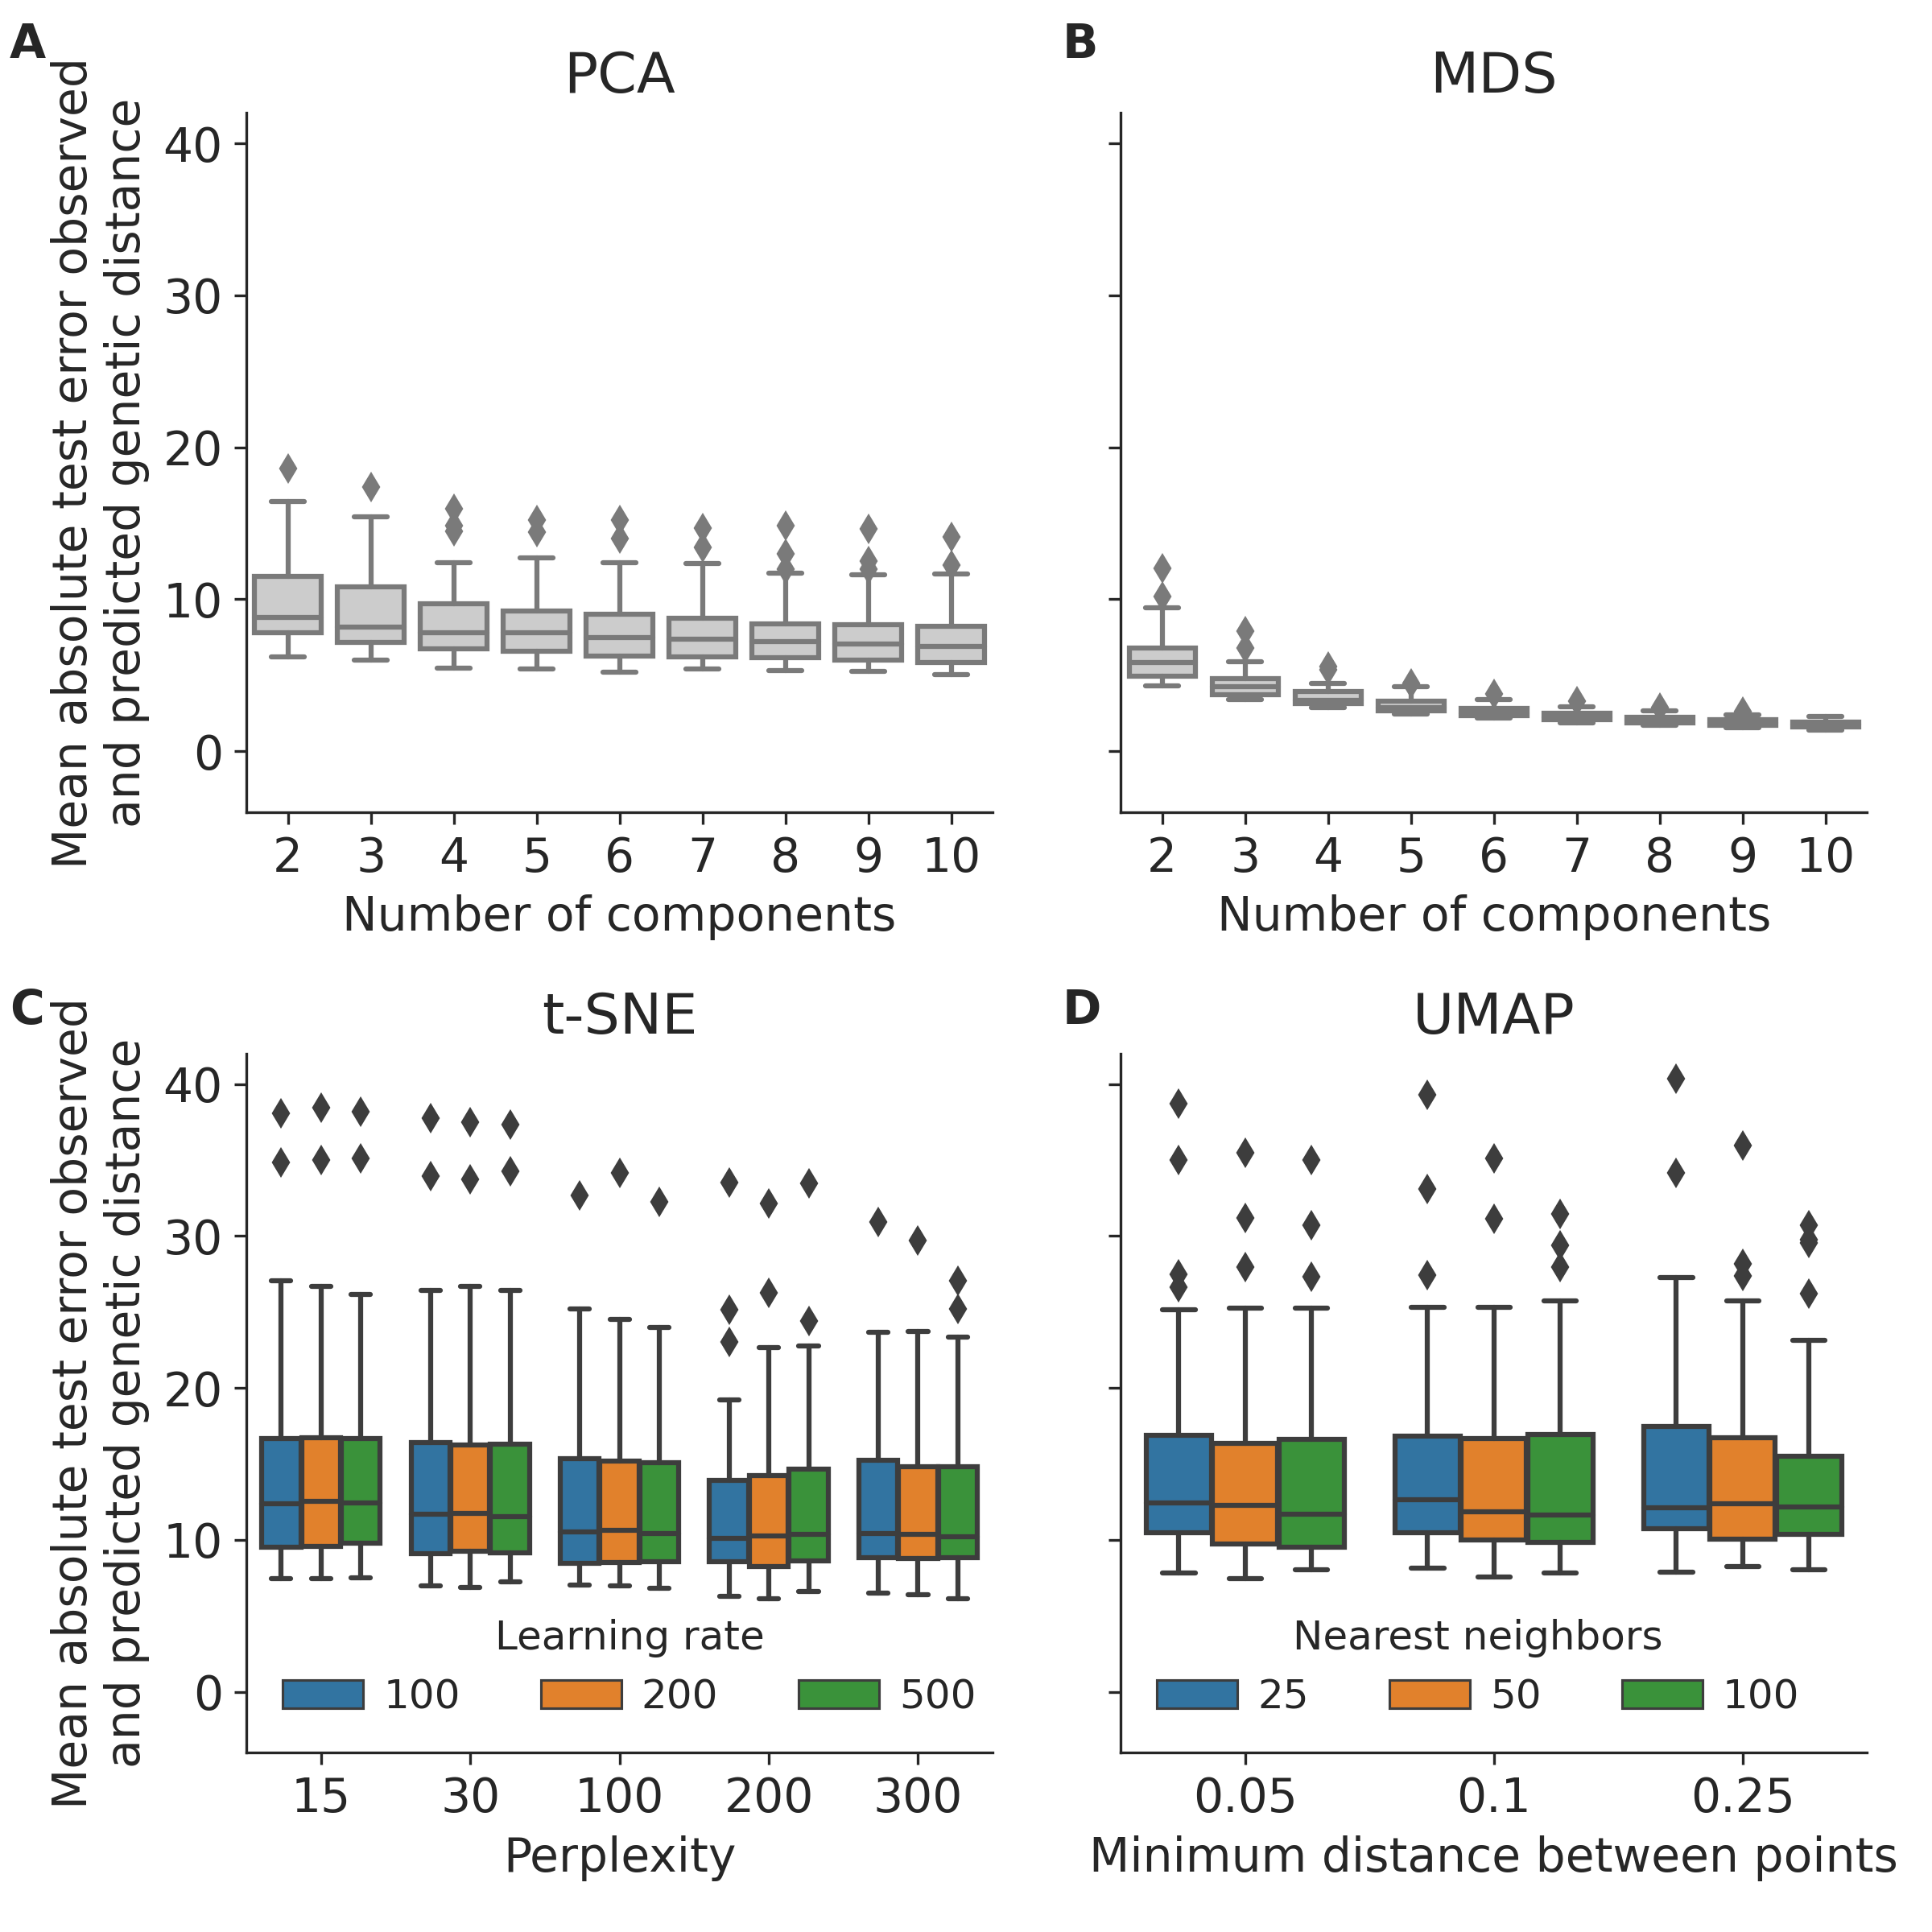
\includegraphics[width=\columnwidth]{figures/simulated-influenza-like-with-no-reassortment-scores-by-parameters.png}
  \caption*{{\bf S1 Fig. Distribution of mean absolute errors (MAE) between observed and predicted pairwise genetic distances per embedding method parameters for simulated influenza-like populations.}}
\end{figure}

% TODO: remove supporting information figures in final submission; figures must be uploaded separately from the manuscript.
\begin{figure}[!h]
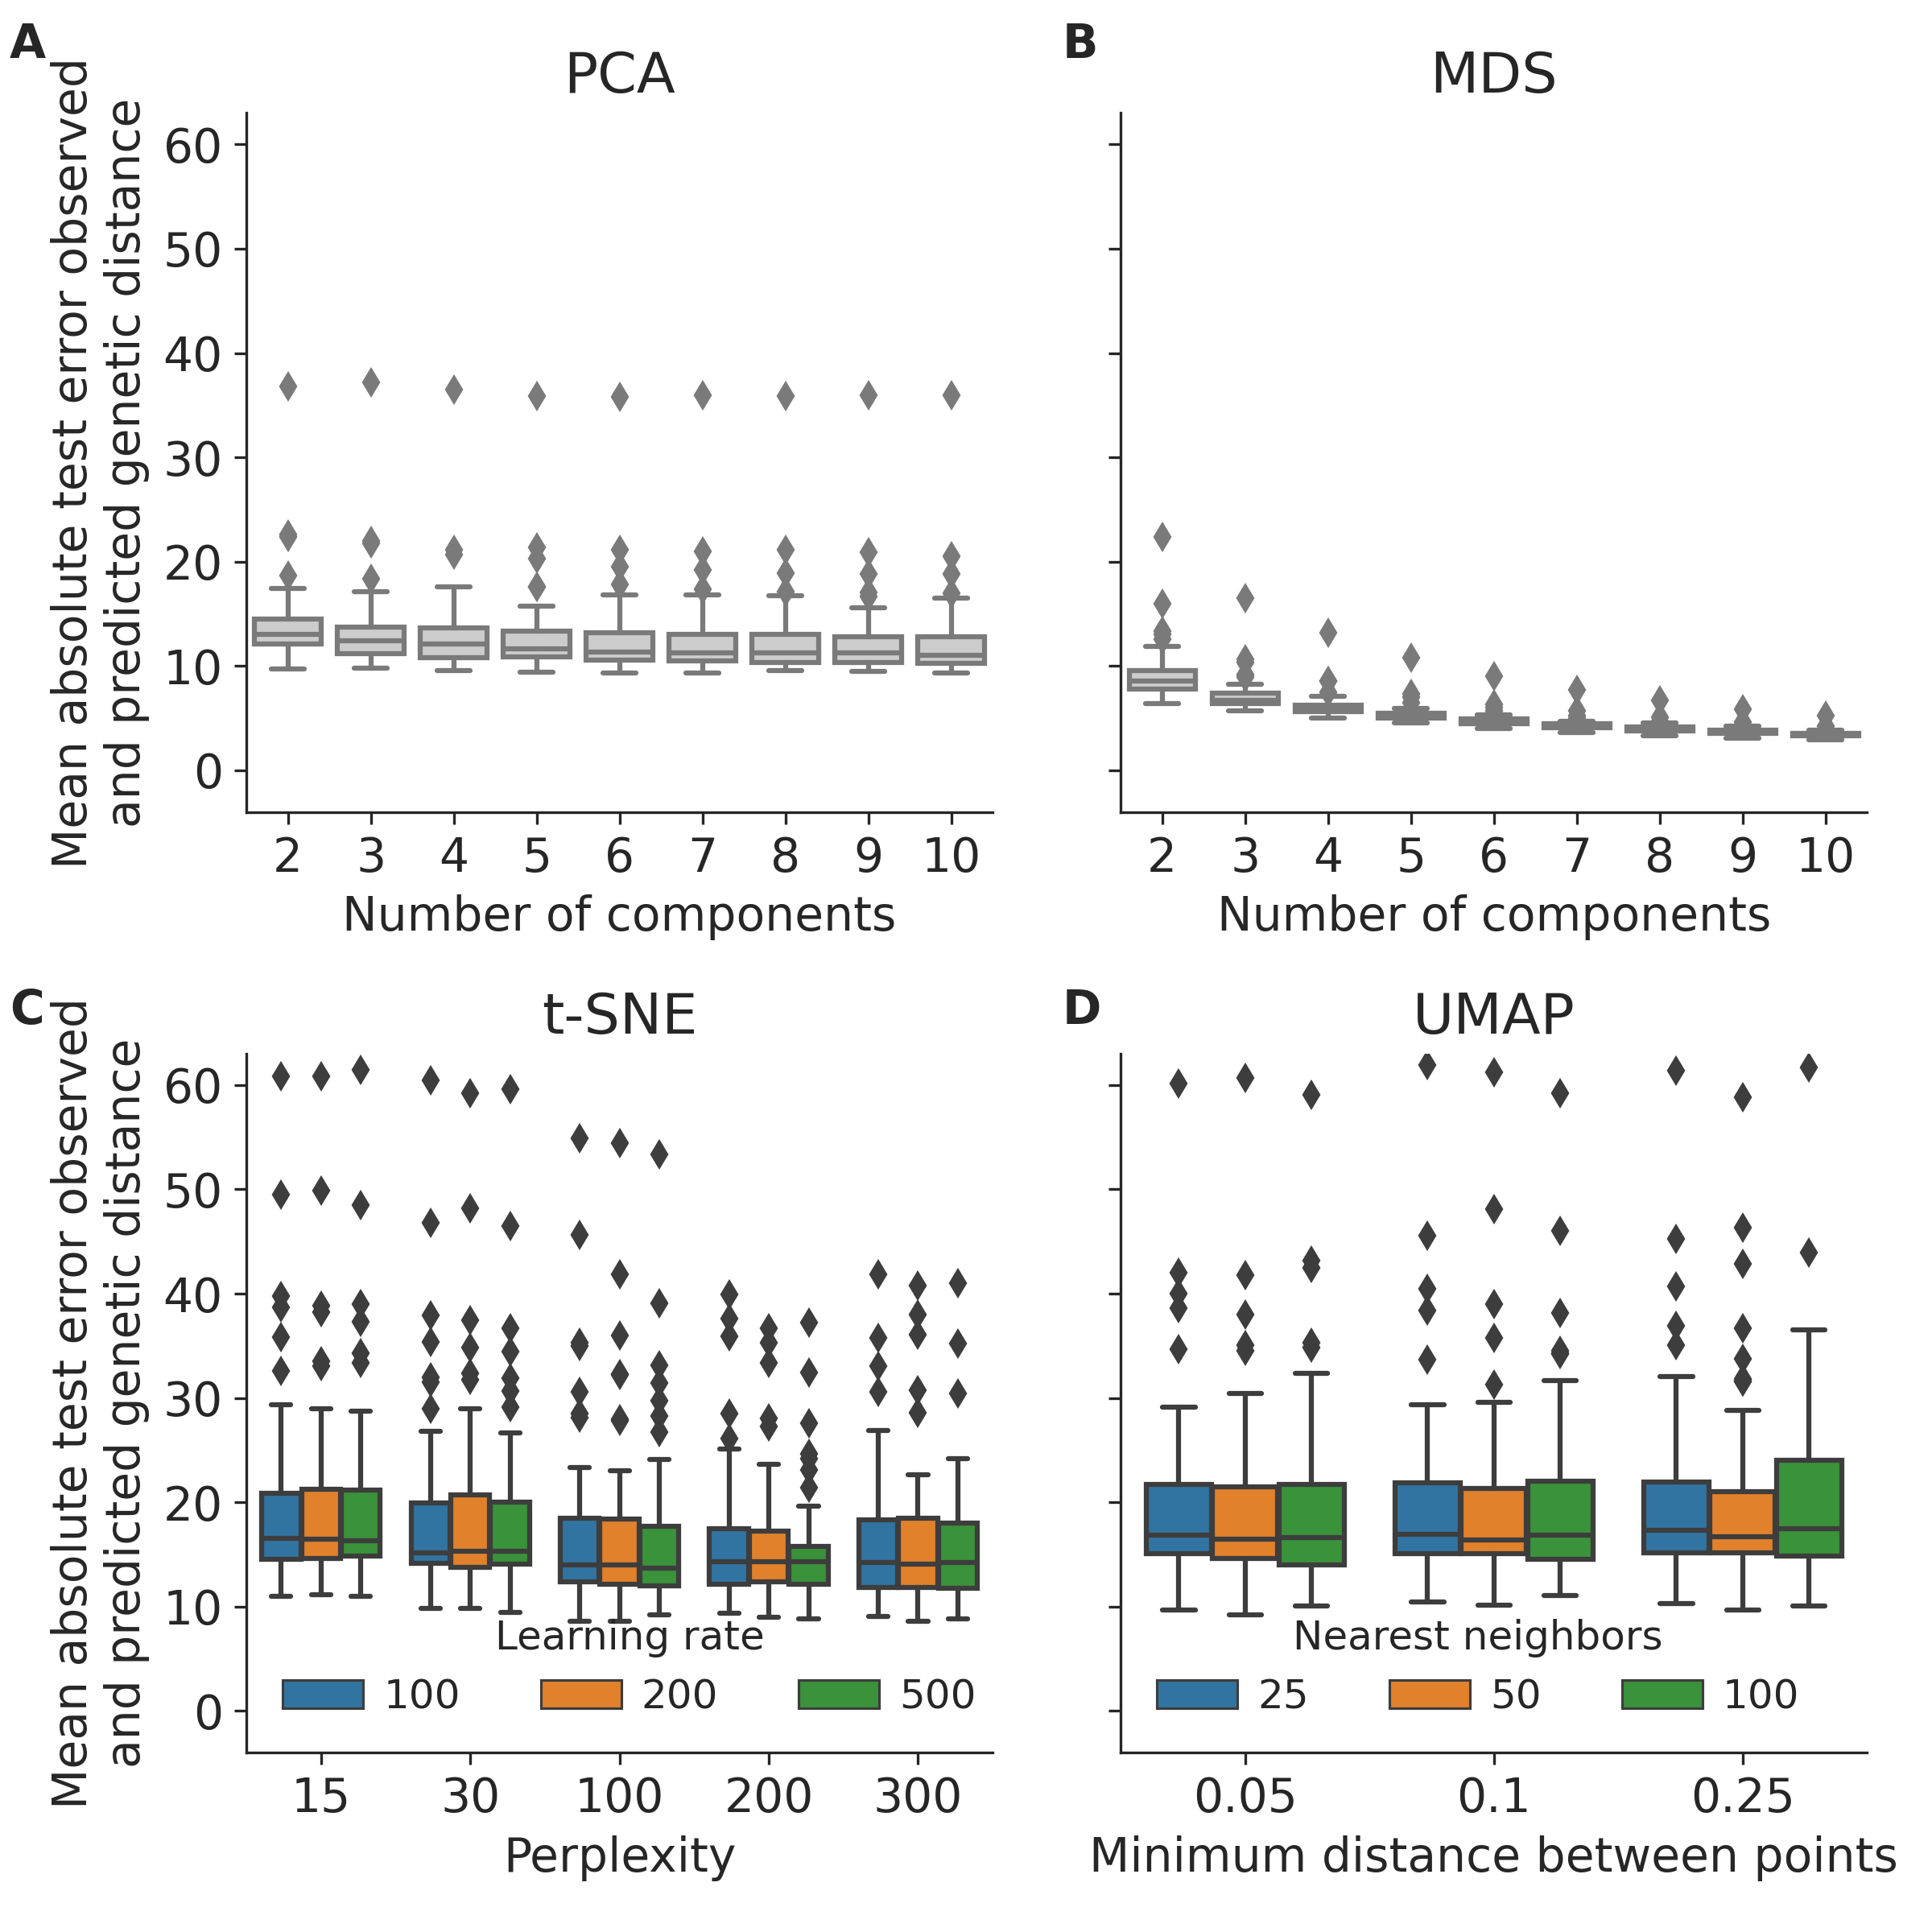
\includegraphics[width=\columnwidth]{figures/simulated-coronavirus-like-with-moderate-recombination-rate-scores-by-parameters.png}
\caption*{{\bf S2 Fig. Distribution of mean absolute errors (MAE) between observed and predicted pairwise genetic distances per embedding method parameters for simulated coronavirus-like populations.}}
\end{figure}

\begin{figure}[!h]
% TODO: remove includegraphics commands in final submission; figures must be uploaded separately from the manuscript.
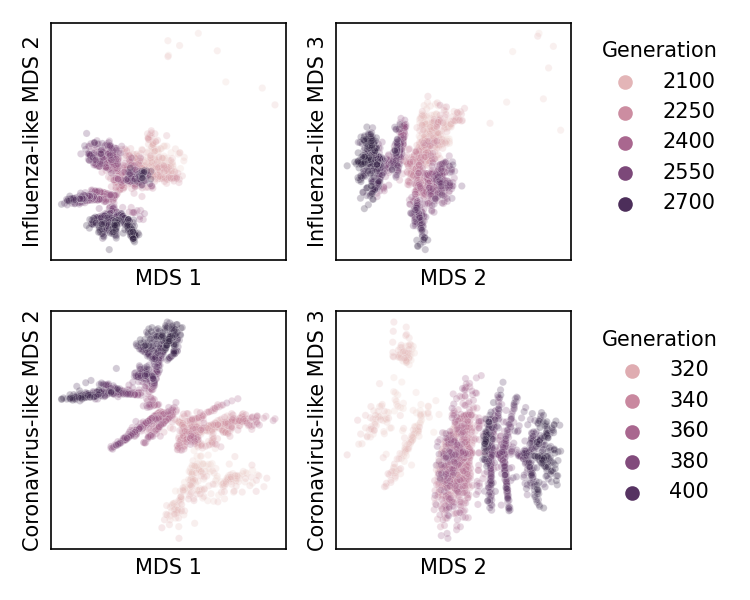
\includegraphics[width=\columnwidth]{figures/simulated-populations-representative-mds-embeddings.png}
\caption*{{\bf S3 Fig. Representative MDS embeddings for simulated populations using optimal parameters per pathogen (rows) and showing all three components.}}
\end{figure}

\begin{figure}[!h]
% TODO: remove includegraphics commands in final submission; figures must be uploaded separately from the manuscript.
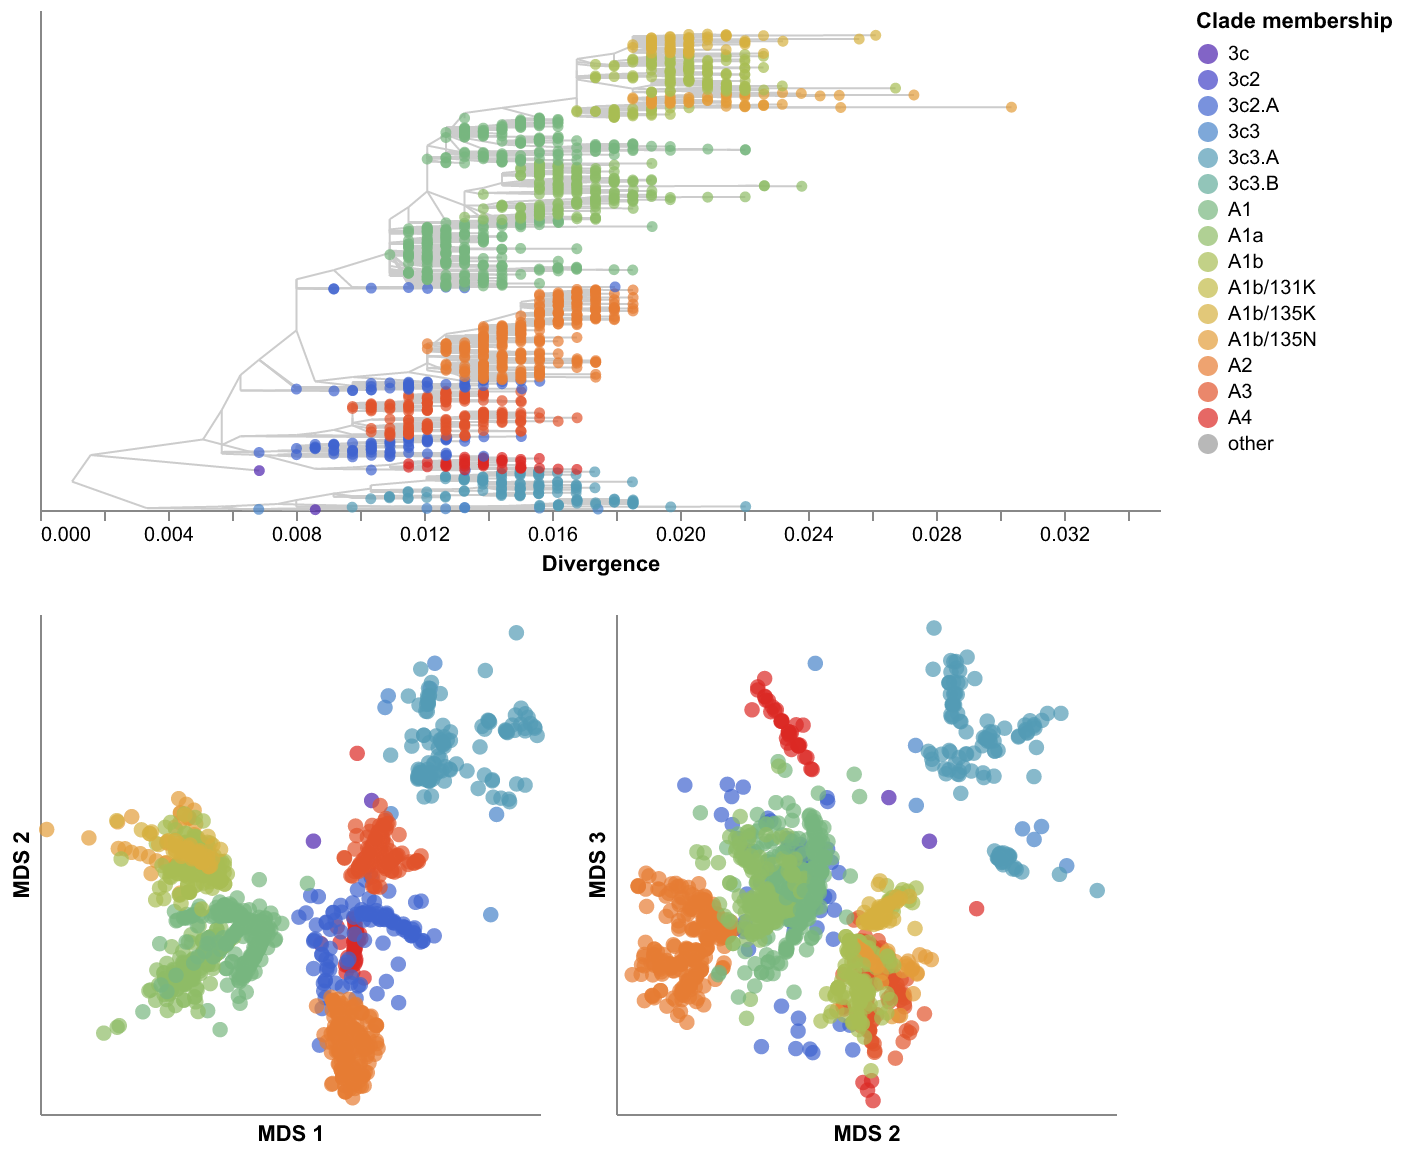
\includegraphics[width=\columnwidth]{figures/flu-2016-2018-mds-by-clade.png}
\caption*{{\bf S4 Fig. MDS embeddings for early (2016--2018) influenza H3N2 HA sequences showing all three components.}
  Line segments in each embedding reflect phylogenetic relationships with internal node positions calculated from the mean positions of their immediate descendants in each dimension (see Methods).
  Line colors represent the clade membership of the most ancestral node in the pair of nodes connected by the segment.
  Line thickness scales by the square root of the number of leaves descending from a given node in the phylogeny.}
\end{figure}

\begin{figure}[!h]
% TODO: remove includegraphics commands in final submission; figures must be uploaded separately from the manuscript.
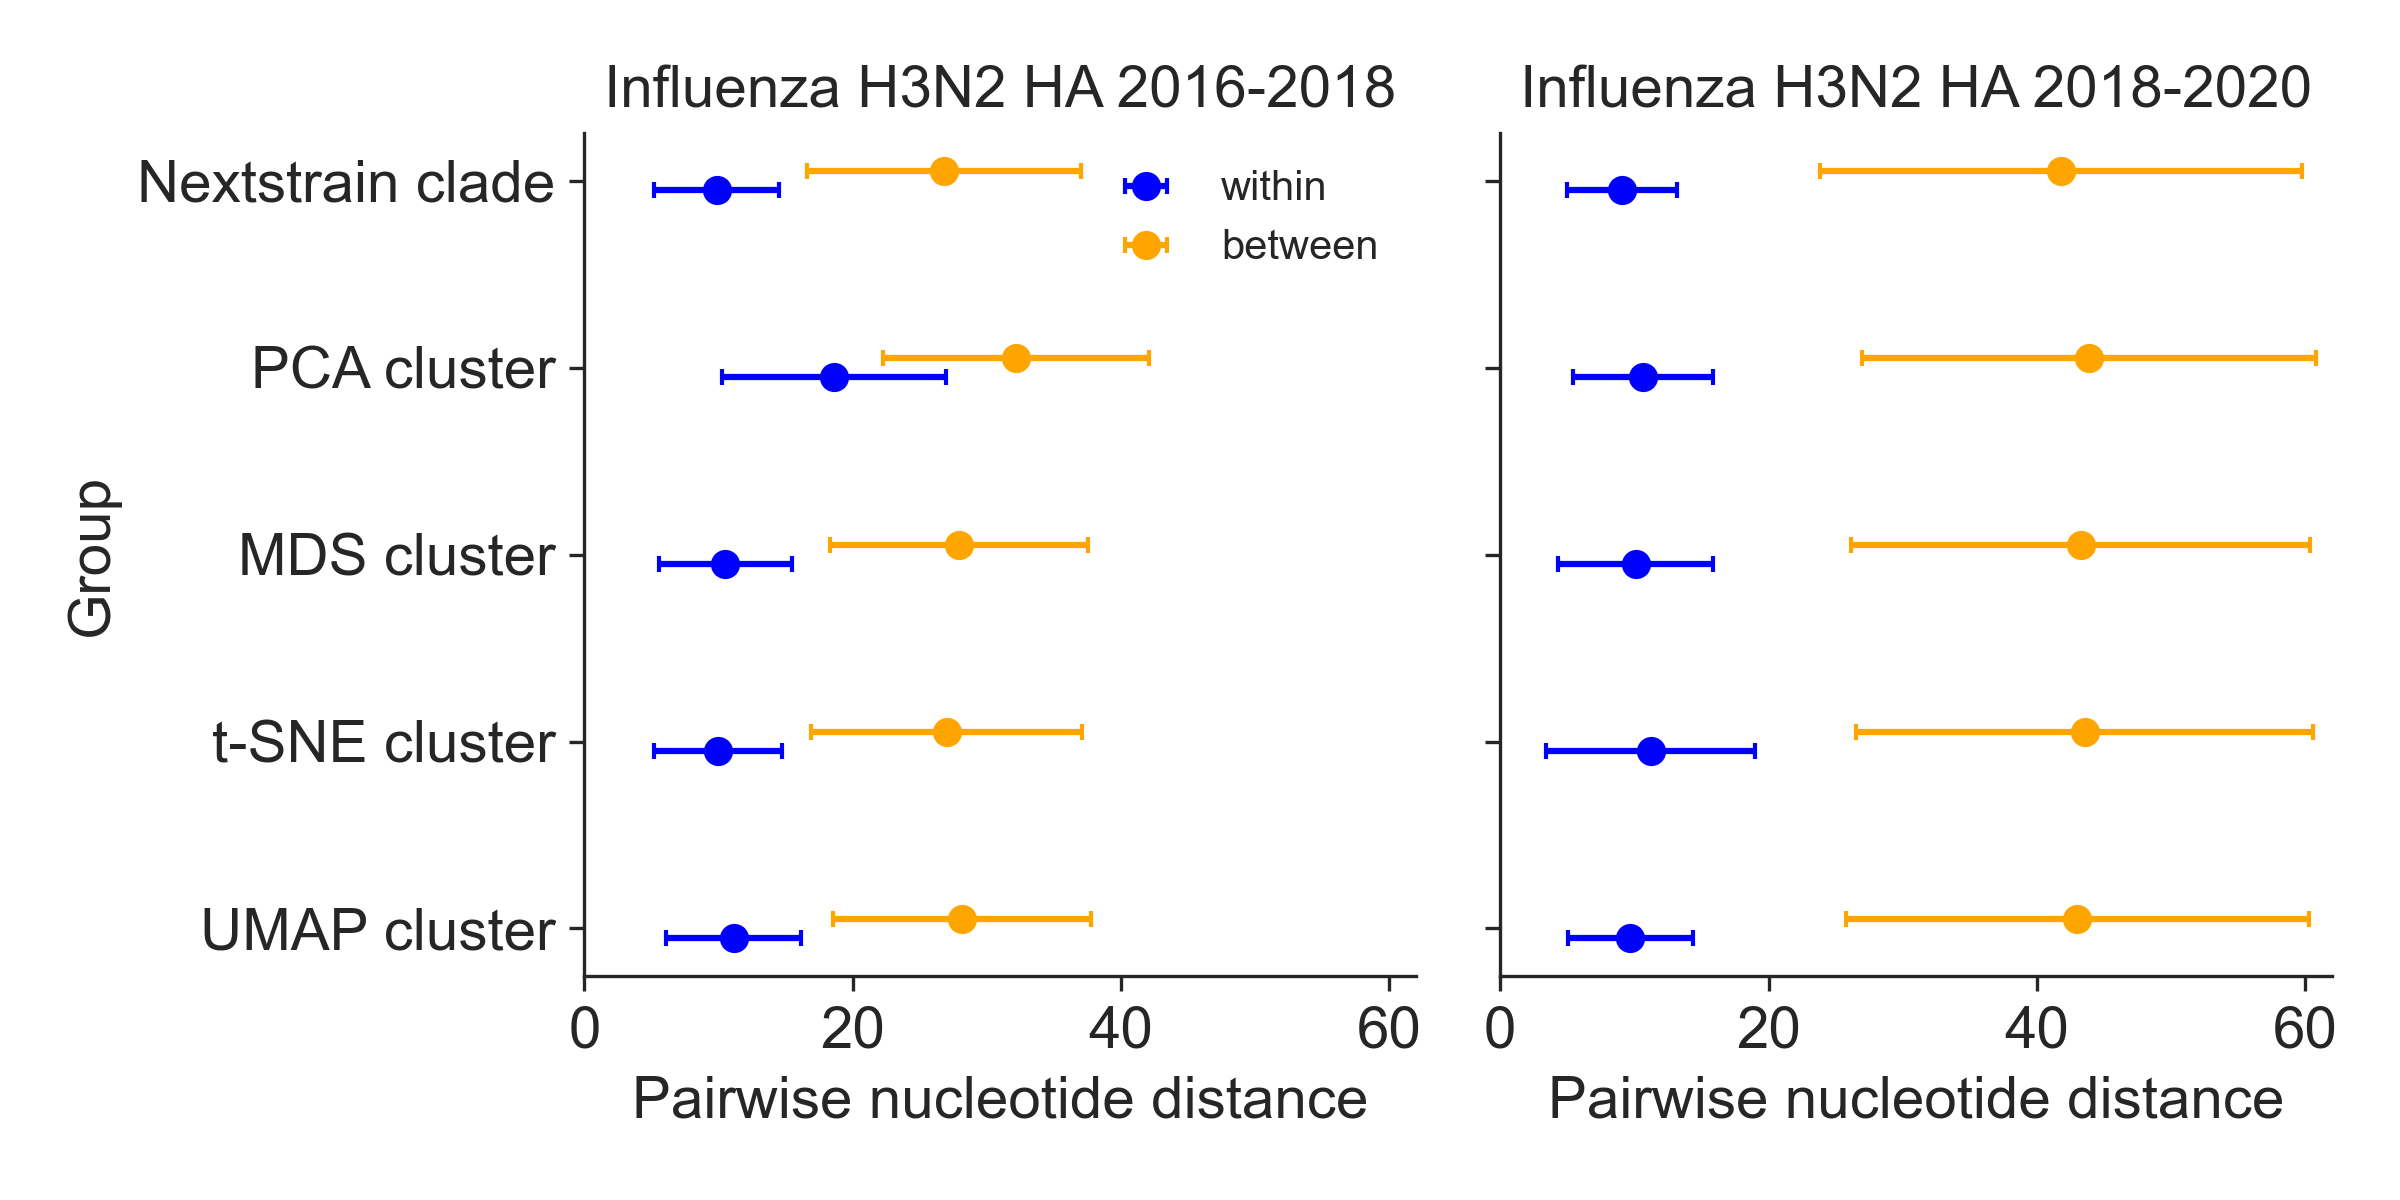
\includegraphics[width=\columnwidth]{figures/within_between_influenza.png}
\caption*{{\bf S5 Fig. Pairwise nucleotide distances for early (2016--2018) and late (2018--2020) influenza H3N2 HA sequences within and between genetic groups defined by Nextstrain clades and clusters from PCA, MDS, t-SNE, and UMAP embeddings.}}
\end{figure}

\begin{figure}[!h]
% TODO: remove includegraphics commands in final submission; figures must be uploaded separately from the manuscript.
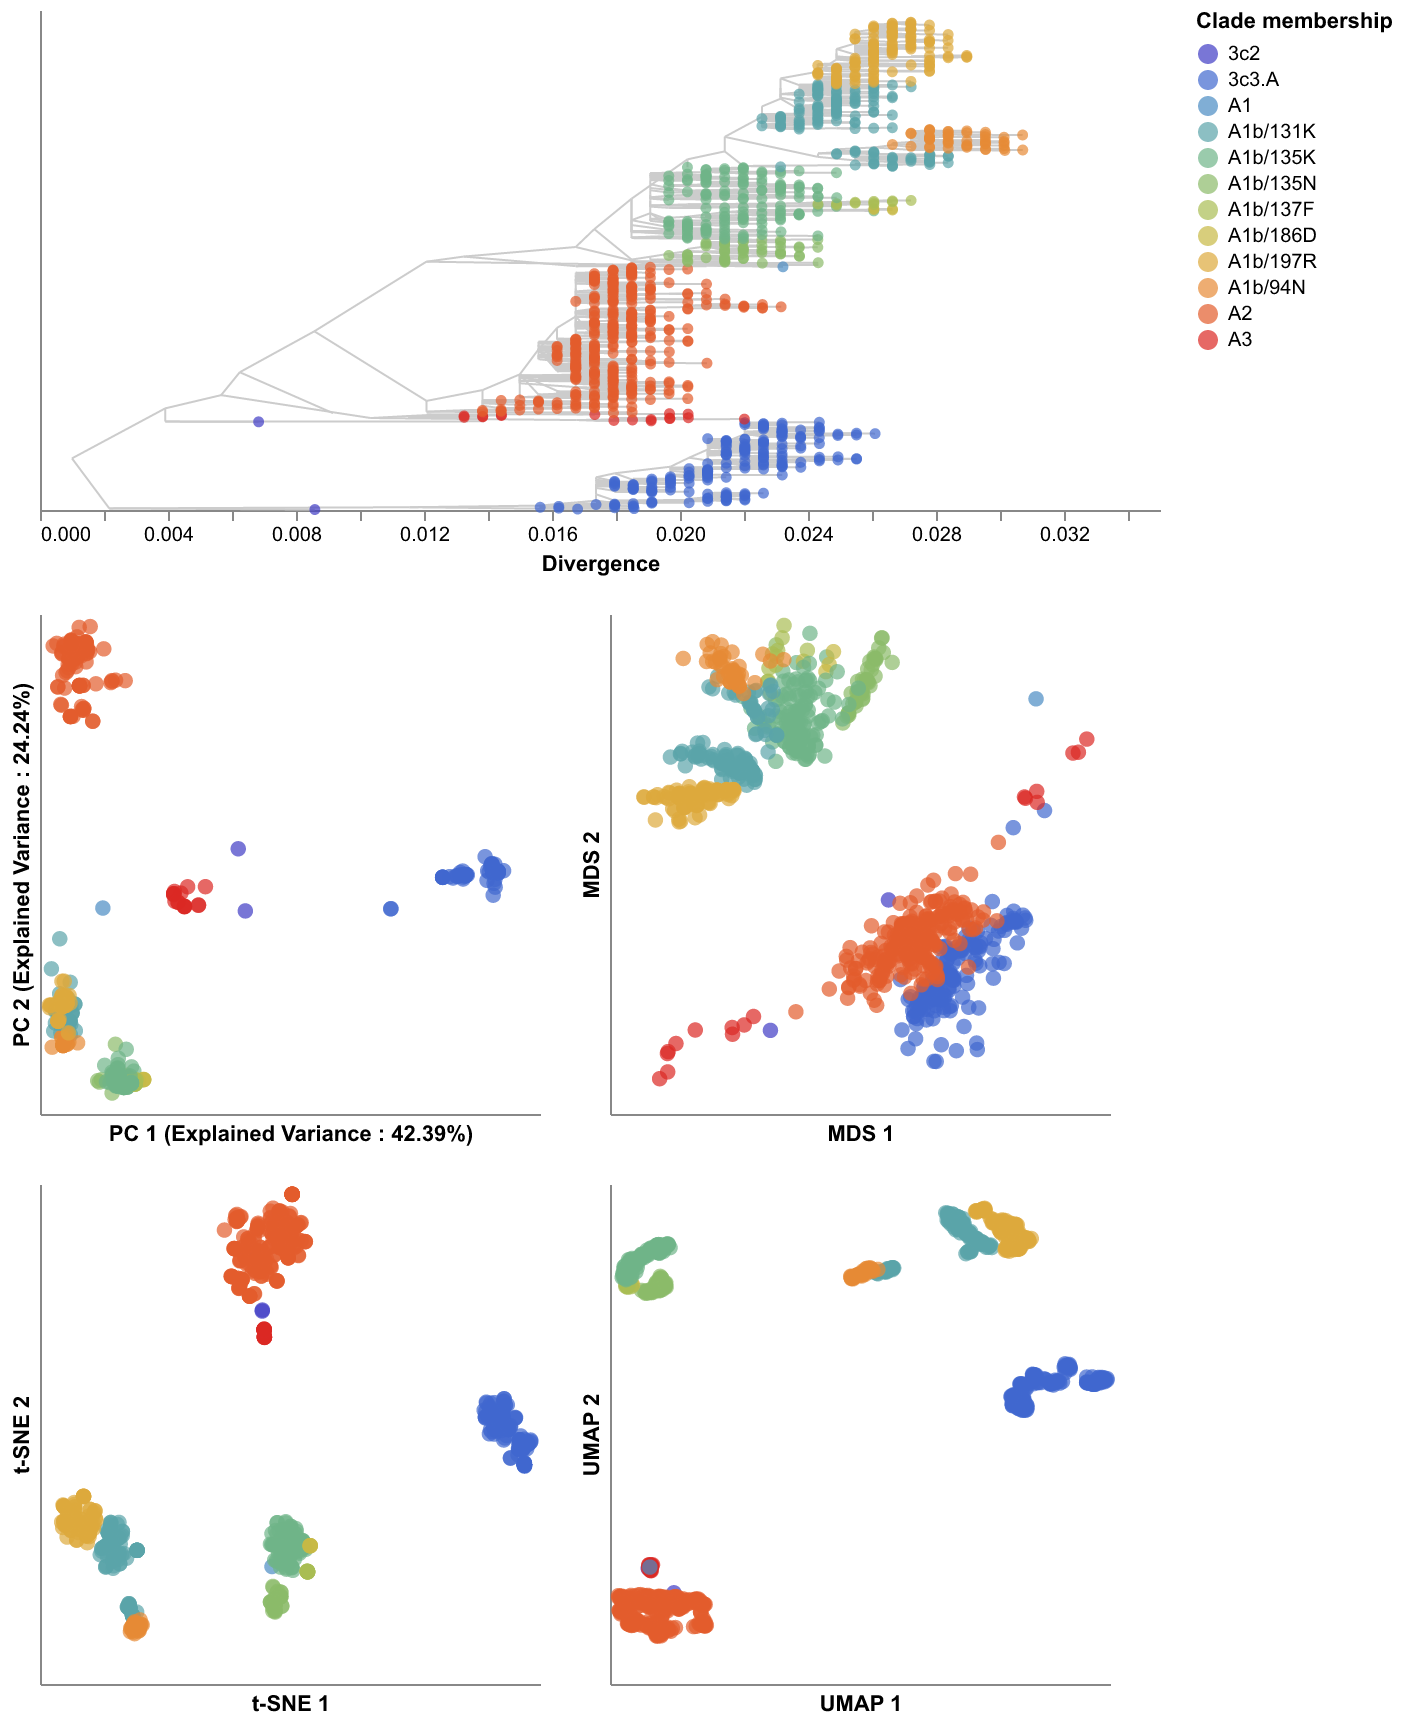
\includegraphics[width=\columnwidth]{figures/flu-2018-2020-ha-embeddings-by-clade.png}
\caption*{{\bf S6 Fig. Phylogeny of late (2018--2020) influenza H3N2 HA sequences plotted by nucleotide substitutions per site on the x-axis (top) and low-dimensional embeddings of the same sequences by PCA (middle left), MDS (middle right), t-SNE (bottom left), and UMAP (bottom right).}
  Tips in the tree and embeddings are colored by their Nextstrain clade assignment.
  Line segments in each embedding reflect phylogenetic relationships with internal node positions calculated from the mean positions of their immediate descendants in each dimension (see Methods).
  Line colors represent the clade membership of the most ancestral node in the pair of nodes connected by the segment.
  Line thickness scales by the square root of the number of leaves descending from a given node in the phylogeny.}
\end{figure}

\begin{figure}[!h]
% TODO: remove includegraphics commands in final submission; figures must be uploaded separately from the manuscript.
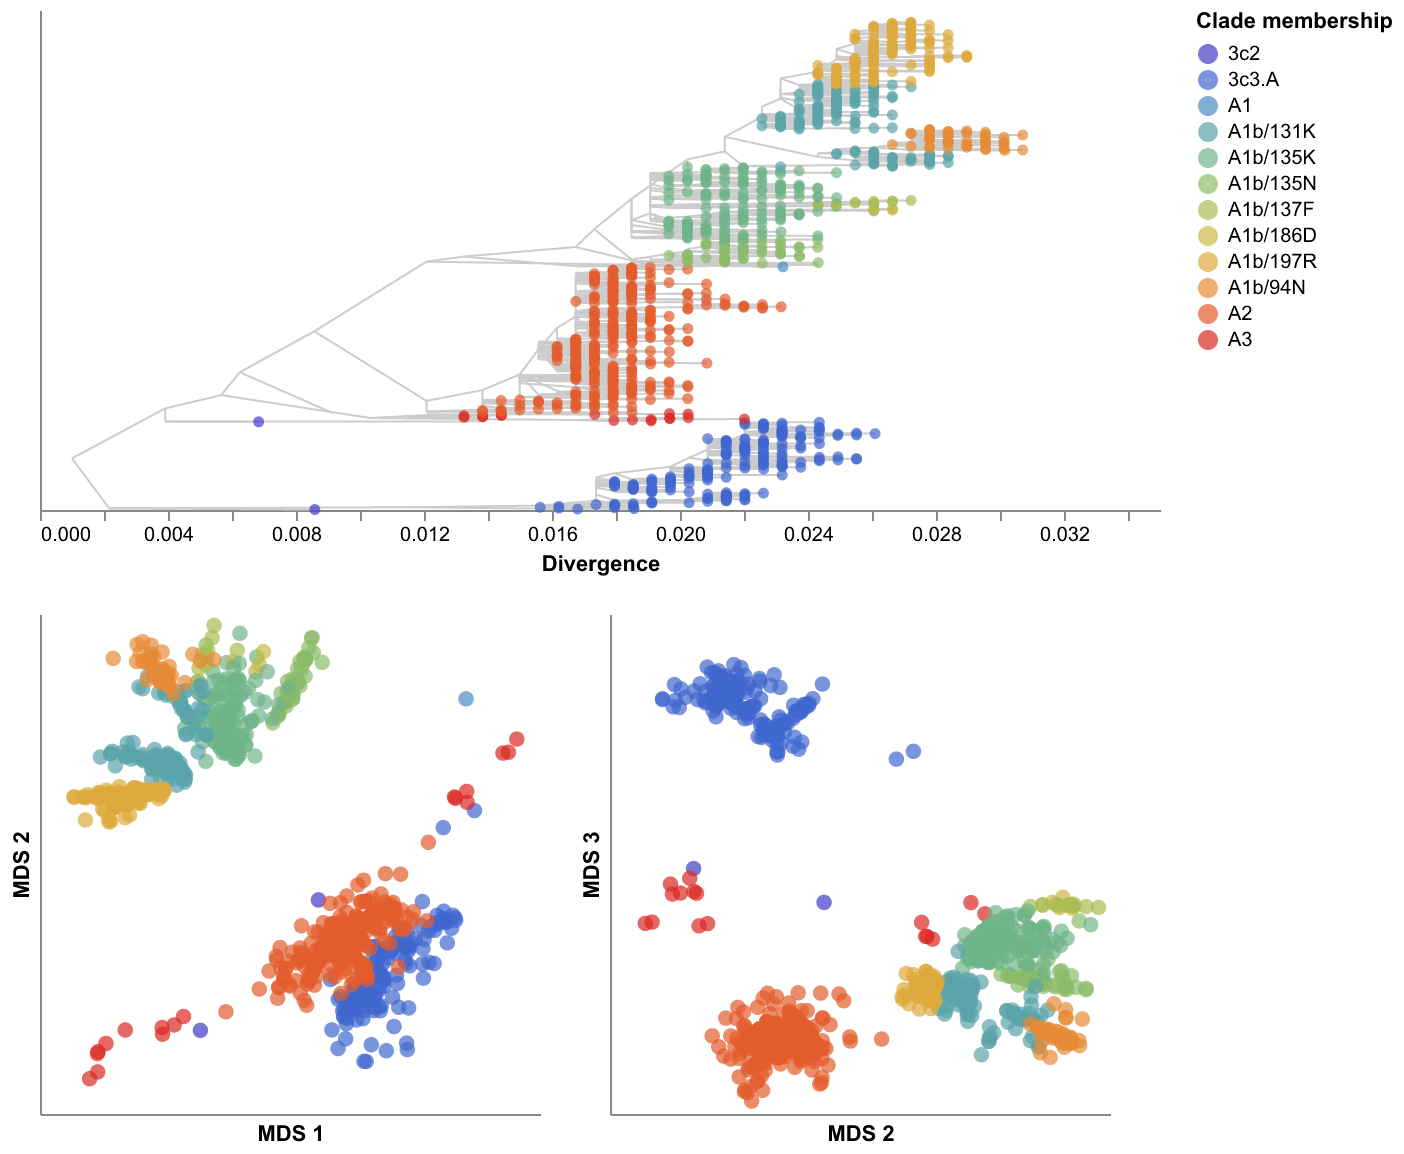
\includegraphics[width=\columnwidth]{figures/flu-2018-2020-mds-by-clade.png}
\caption*{{\bf S7 Fig. MDS embeddings for late (2018--2020) influenza H3N2 HA sequences showing all three components.}
  Line segments in each embedding reflect phylogenetic relationships with internal node positions calculated from the mean positions of their immediate descendants in each dimension (see Methods).
  Line colors represent the clade membership of the most ancestral node in the pair of nodes connected by the segment.
  Line thickness scales by the square root of the number of leaves descending from a given node in the phylogeny.}
\end{figure}

\begin{figure}[!h]
% TODO: remove includegraphics commands in final submission; figures must be uploaded separately from the manuscript.
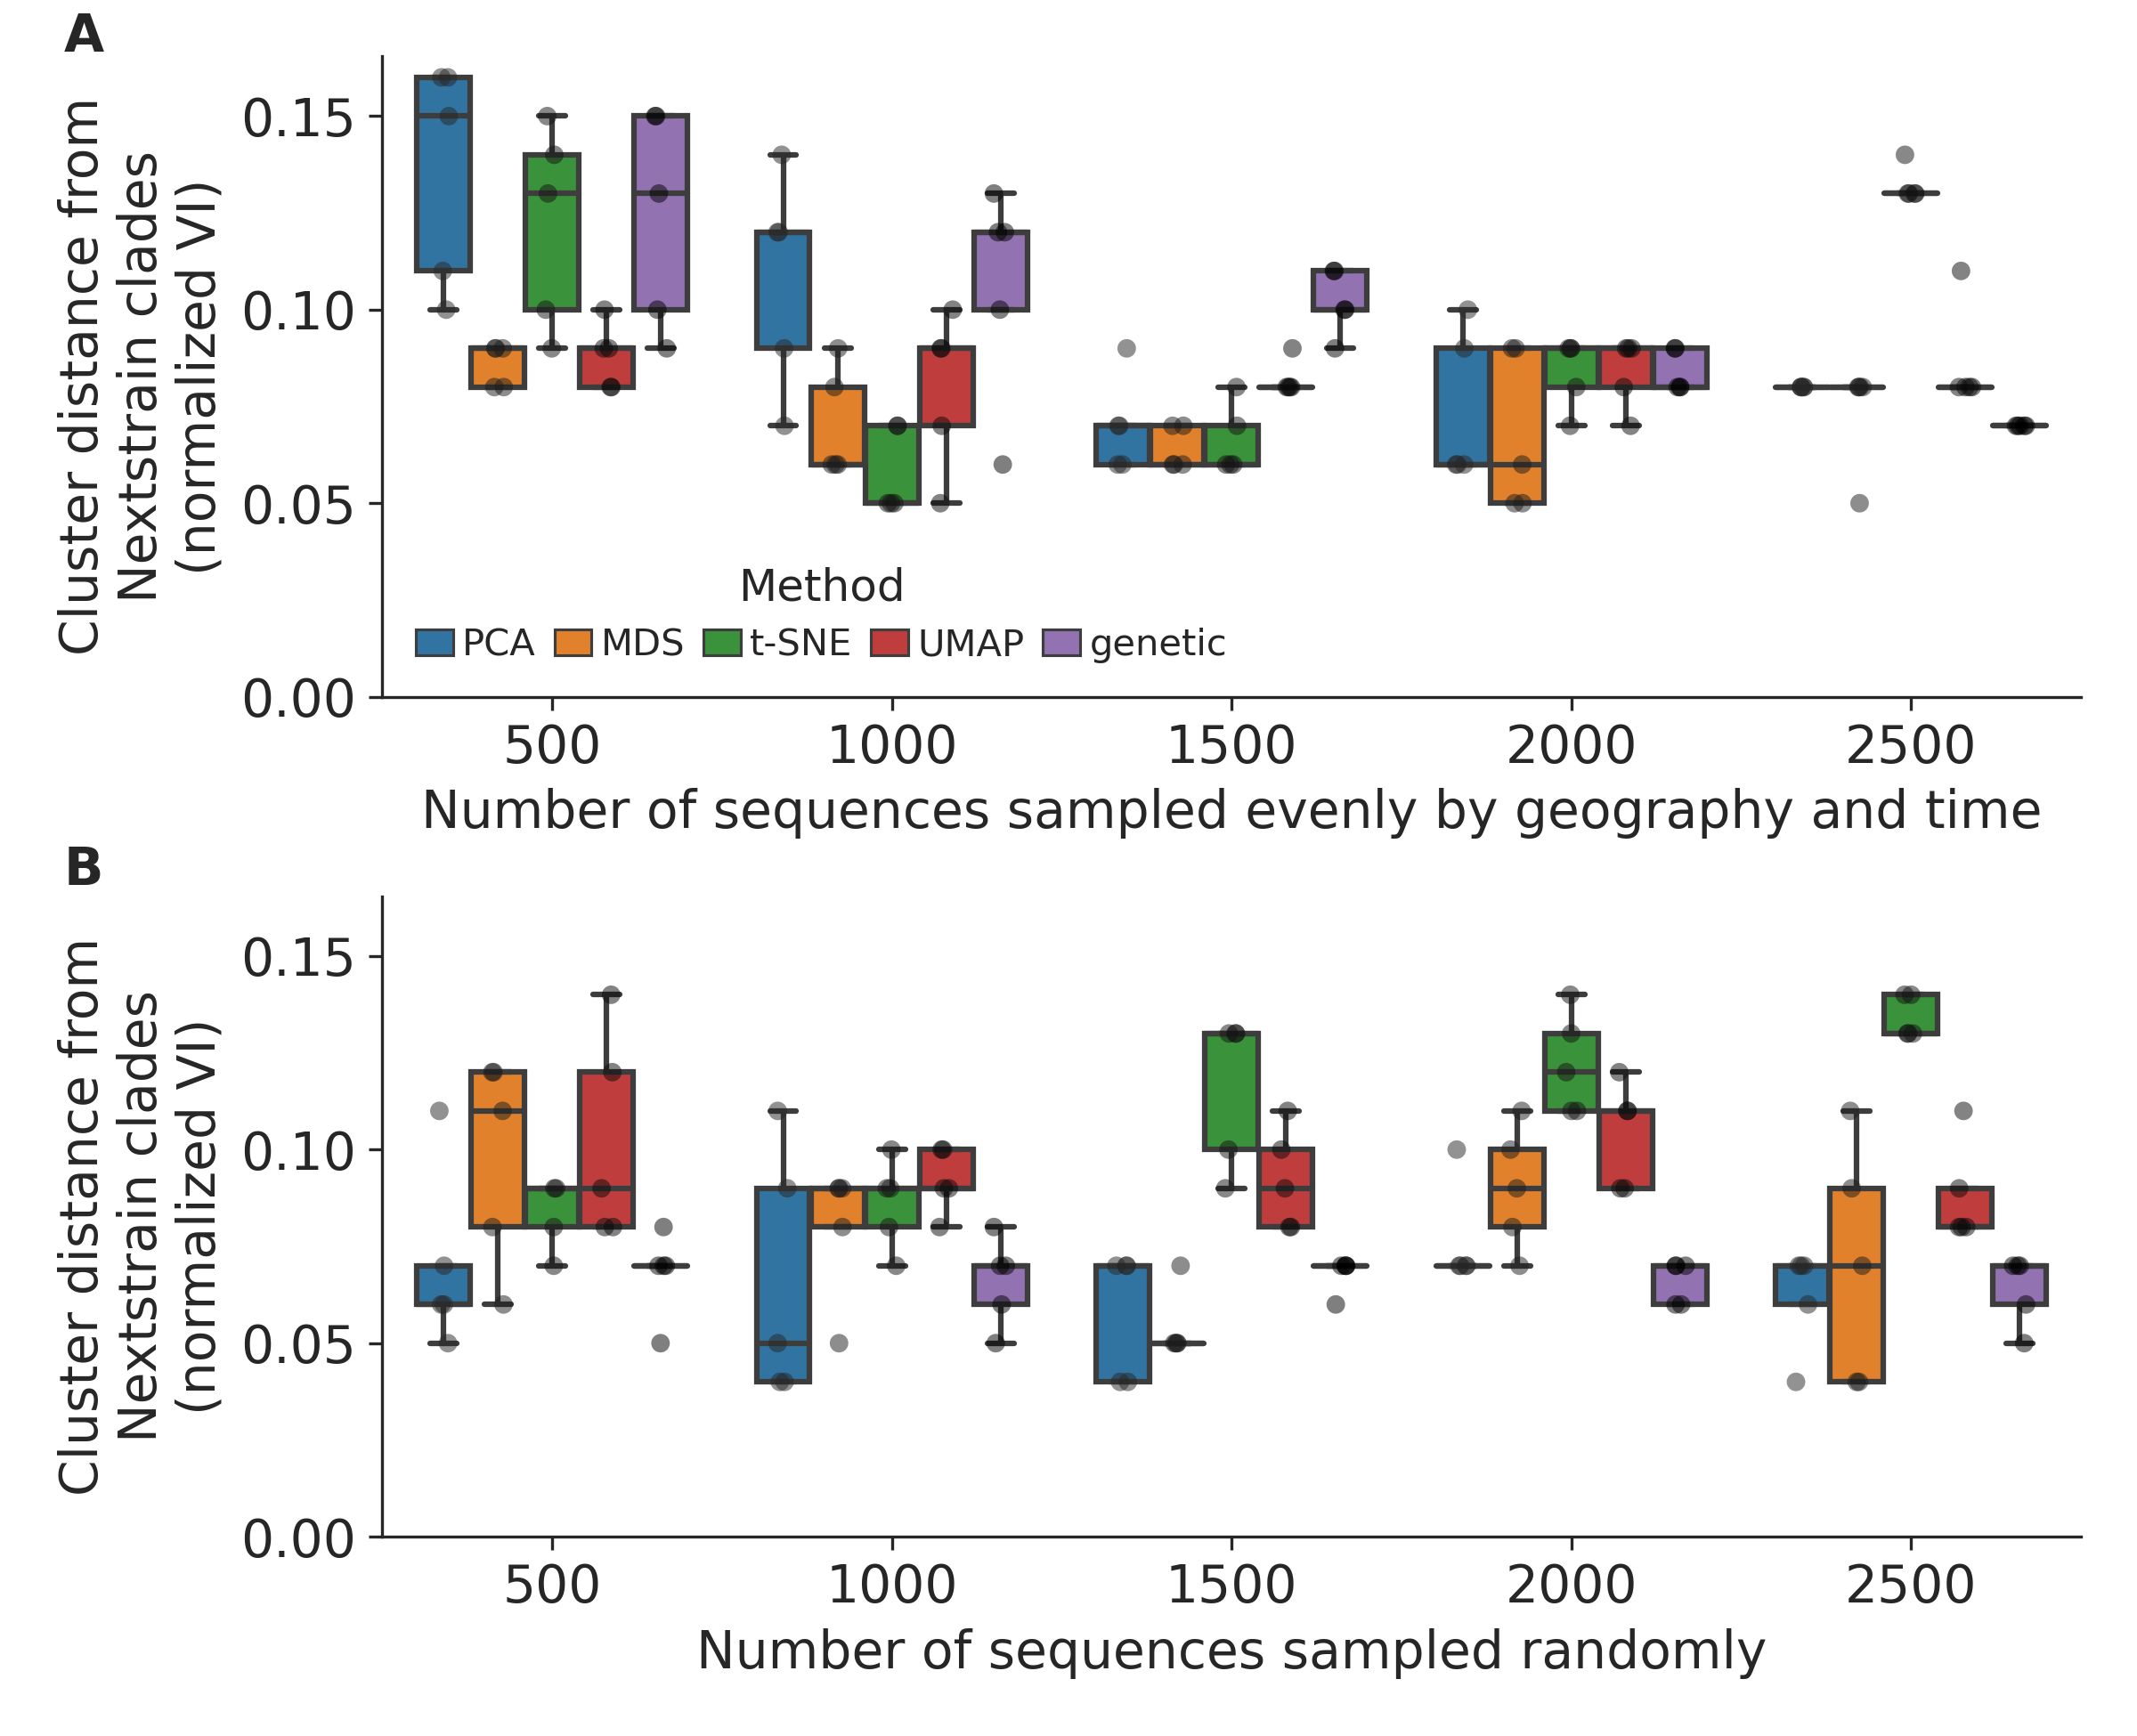
\includegraphics[width=\columnwidth]{figures/flu-2018-2020-replication-of-cluster-accuracy.png}
\caption*{{\bf S8 Fig. Replication of cluster accuracy per embedding method for late (2018--2020) influenza H3N2 HA sequences across different sampling densities (total sequences sampled) and sampling schemes including A) even geographic and temporal sampling and B) random sampling.}
  We measured cluster accuracy across five replicates per sampling density and scheme with the normalized VI distance between clusters from a given embedding and Nextstrain clades for the same samples.
  The even sampling scheme selected sequences evenly across country, year, and month to minimize geographic and temporal bias.
  The random sampling scheme uniformly sampled from the original dataset, reflecting the geographic and genetic bias in those data.
}
\end{figure}

\begin{figure}[!h]
% TODO: remove includegraphics commands in final submission; figures must be uploaded separately from the manuscript.
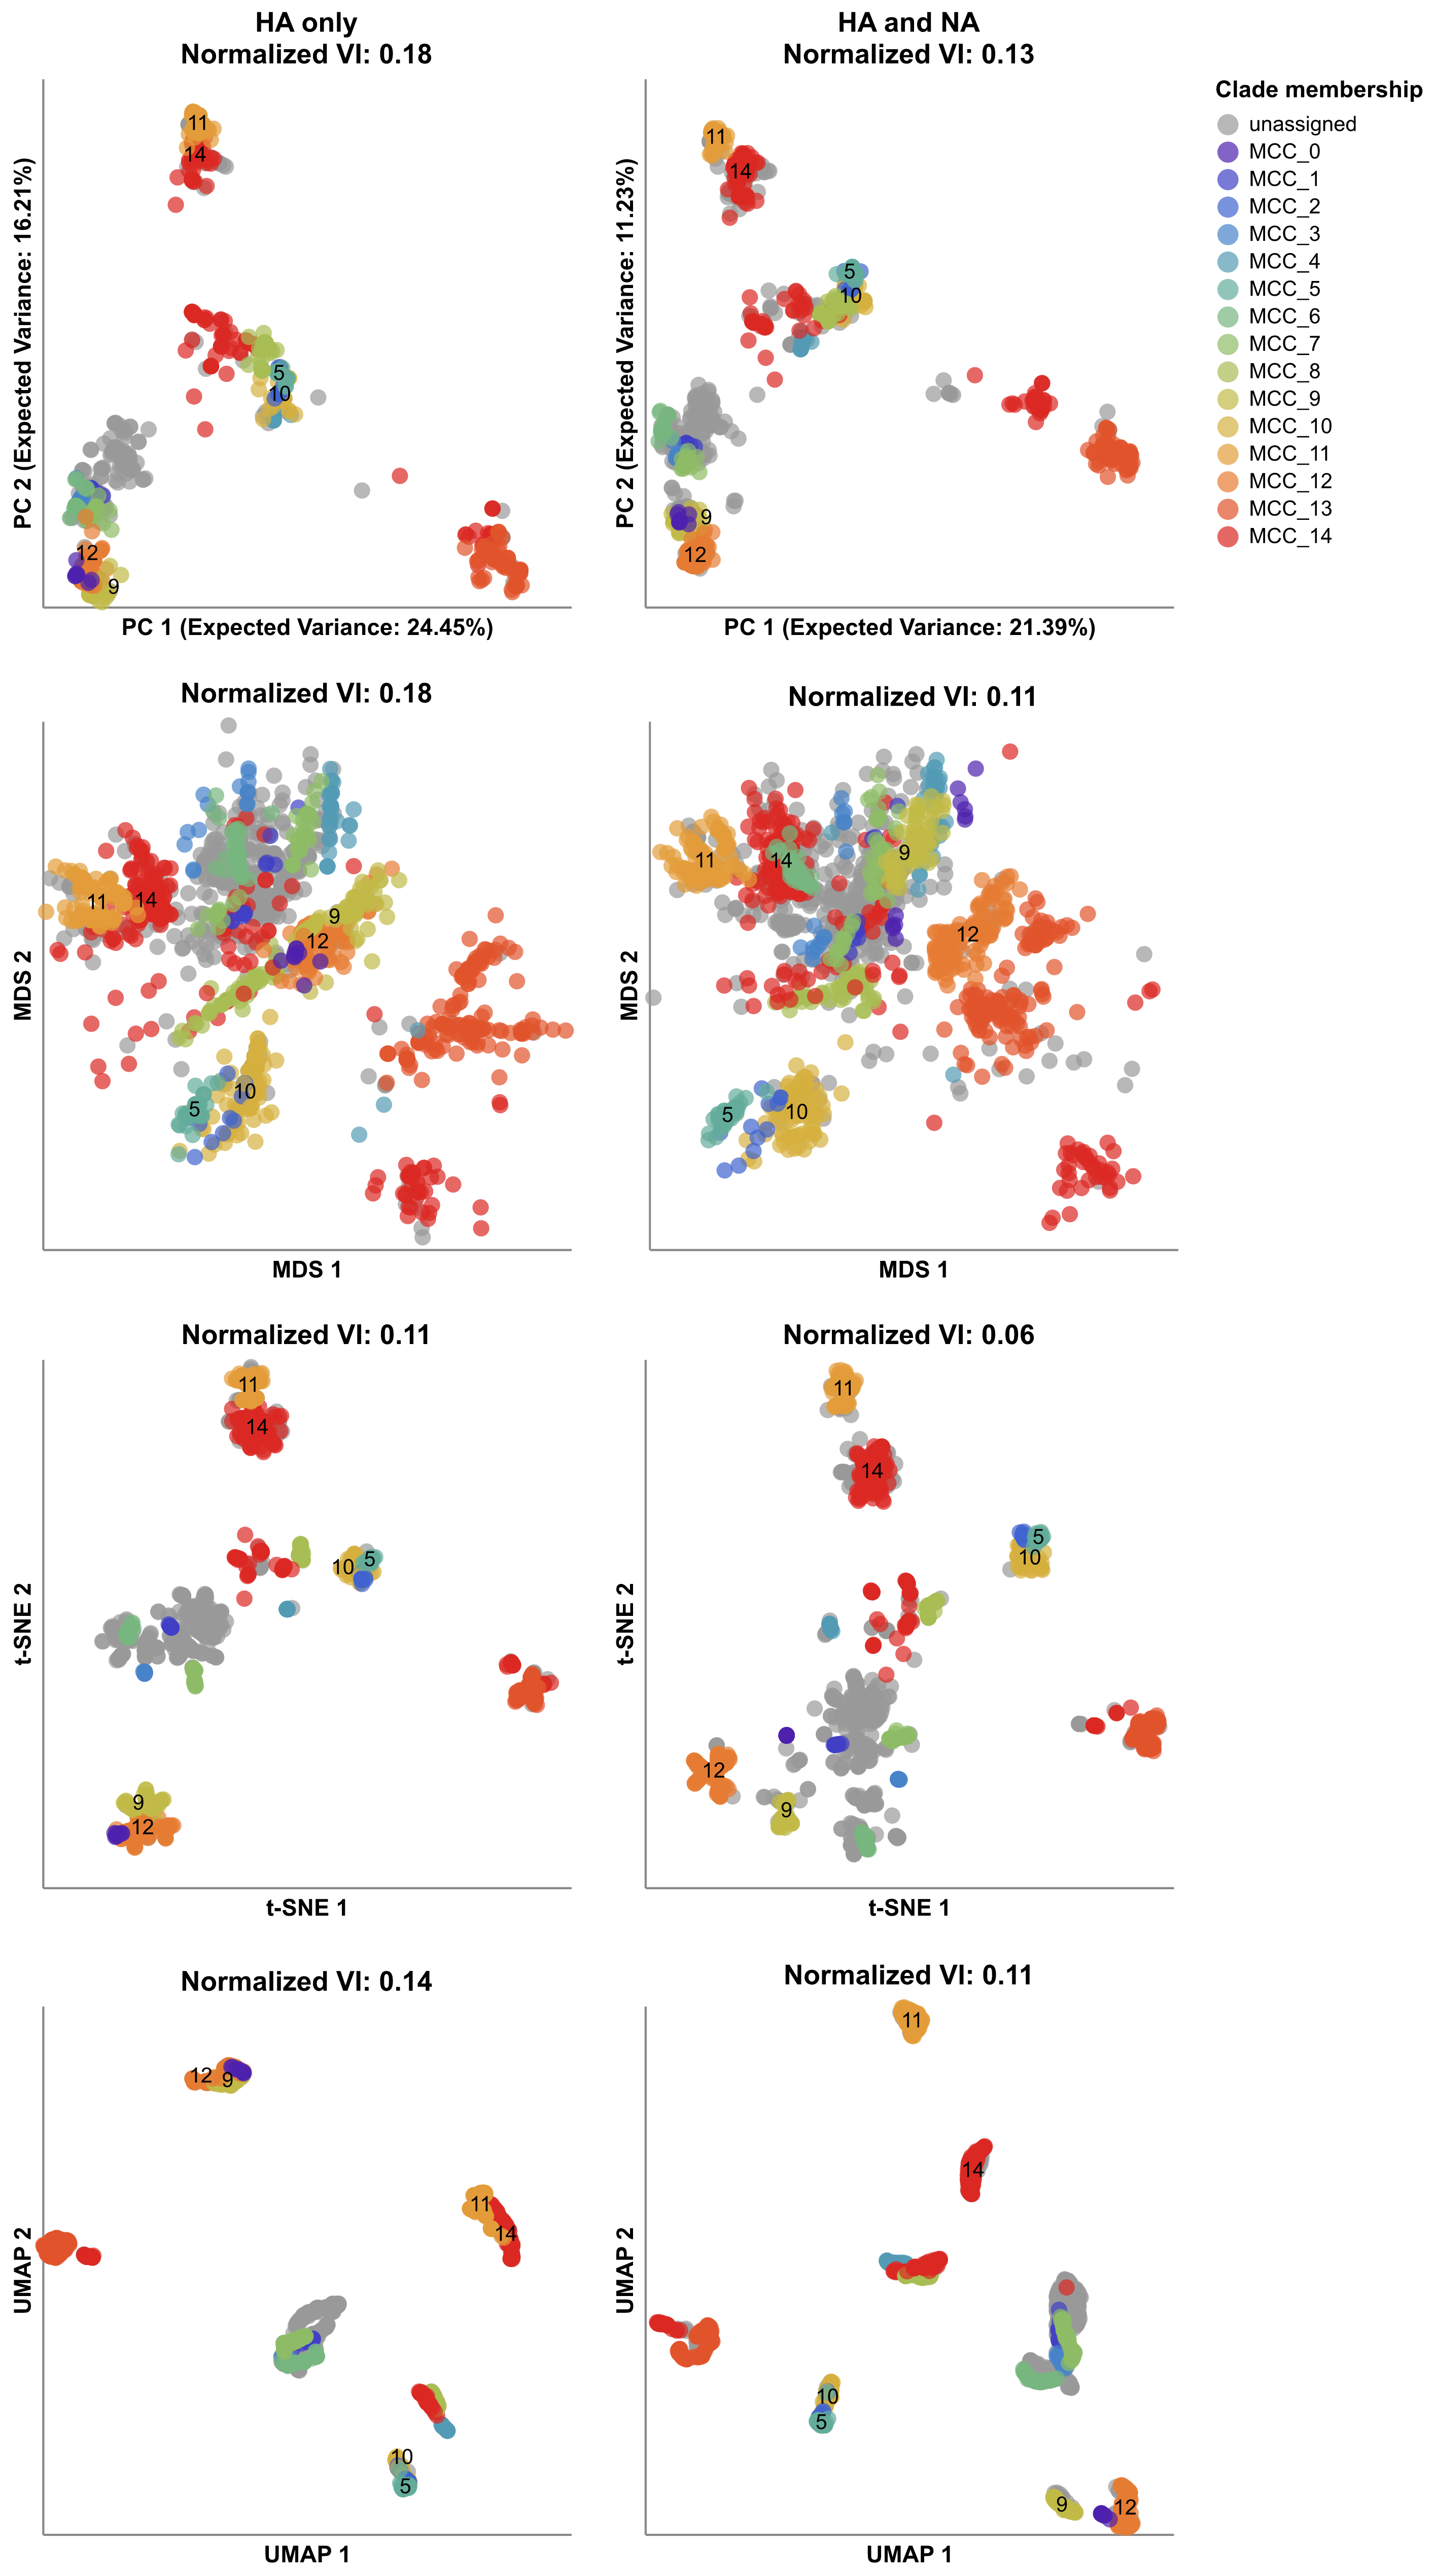
\includegraphics[width=0.75\columnwidth]{figures/flu-2016-2018-ha-na-all-embeddings-by-mcc.png}
\caption*{{\bf S9 Fig. Embeddings influenza H3N2 HA-only (left) and combined HA/NA (right) showing the effects of additional NA genetic information on the placement of reassortment events detected by TreeKnit (MCCs).}}
\end{figure}

\begin{figure}[!h]
% TODO: remove includegraphics commands in final submission; figures must be uploaded separately from the manuscript.
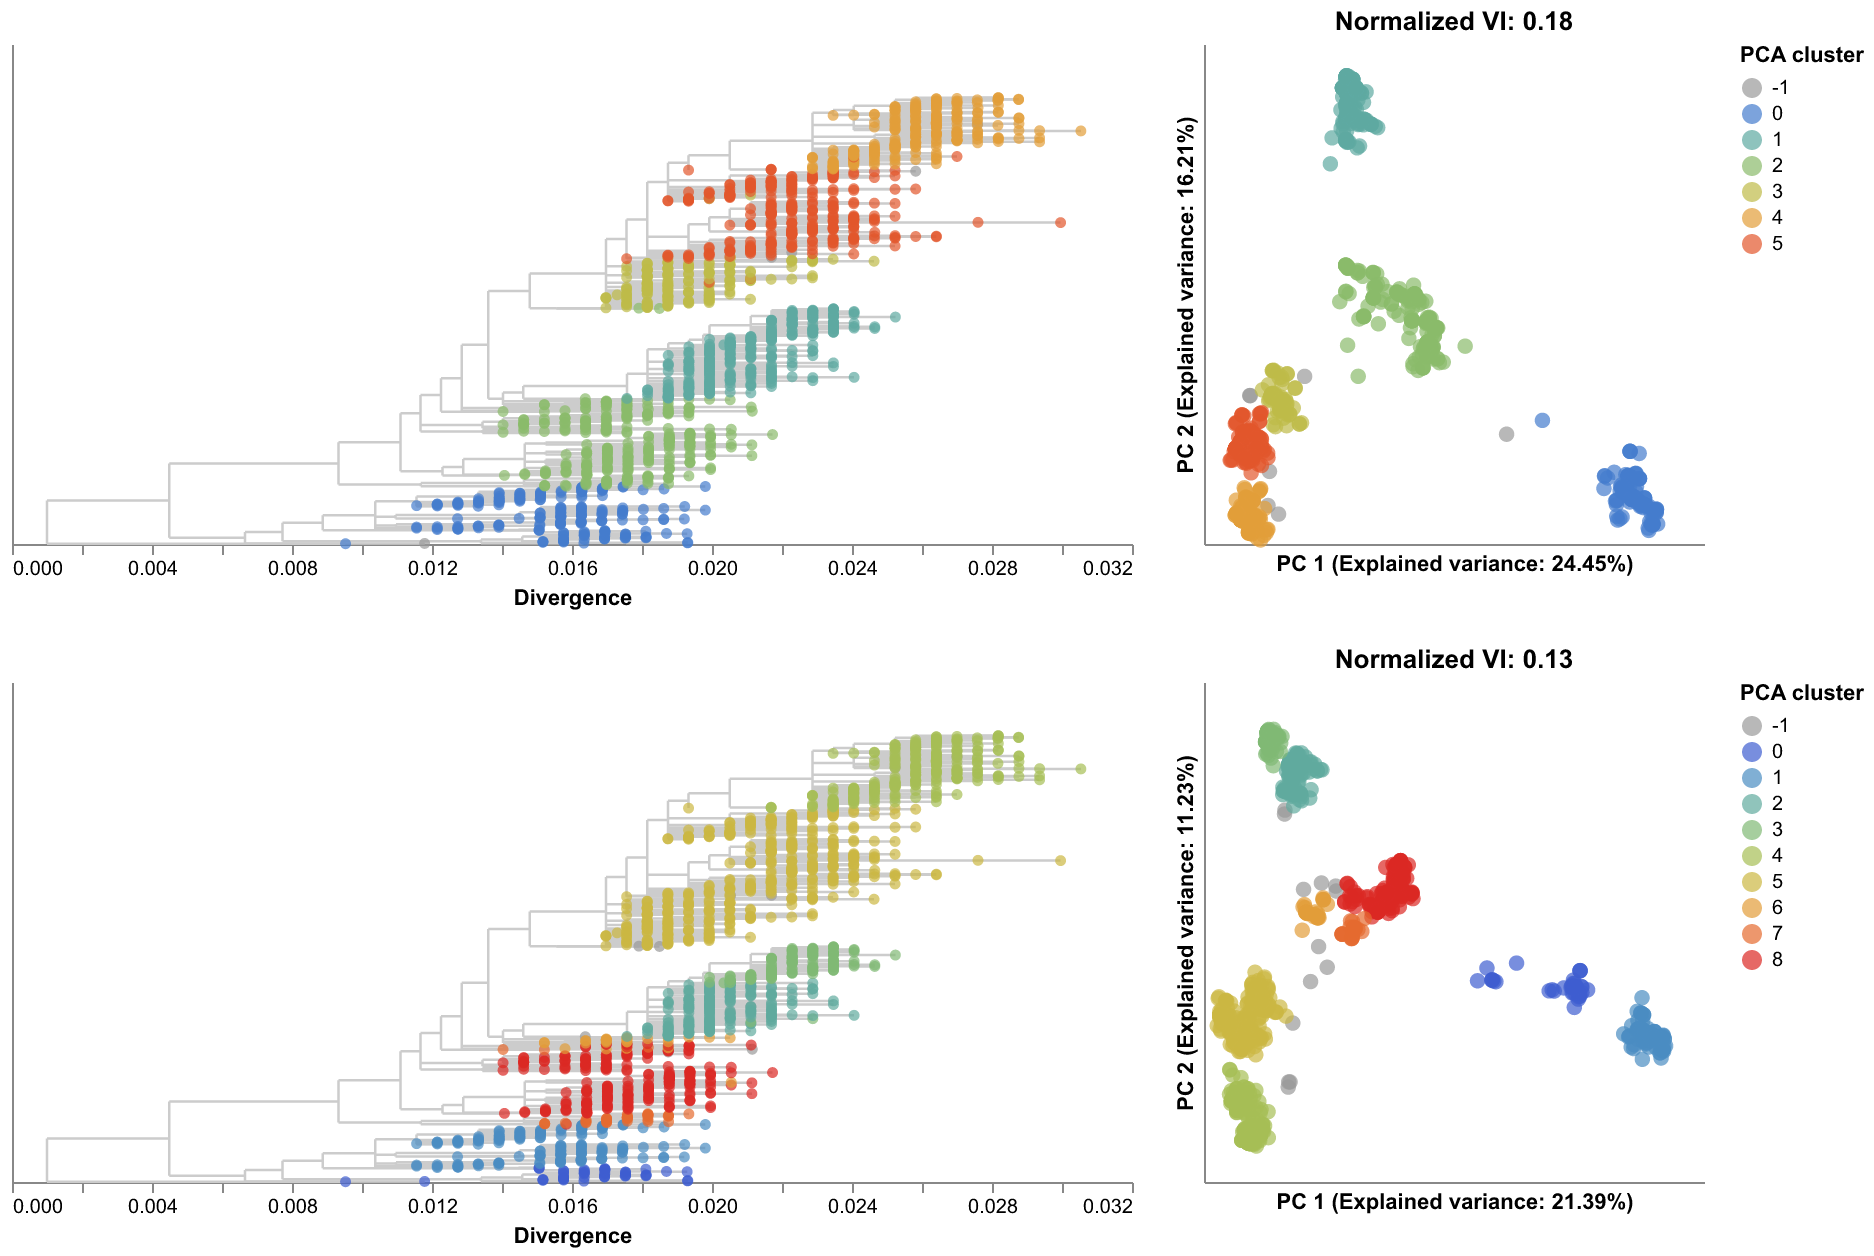
\includegraphics[width=\columnwidth]{figures/flu-2016-2018-ha-na-pca-by-cluster.png}
\caption*{{\bf S10 Fig. PCA embeddings for influenza H3N2 HA sequences only (top row) and HA/NA sequences combined (bottom row) showing the HA trees colored by clusters identified in each embedding (left) and the corresponding embeddings colored by cluster (right).}}
\end{figure}

\begin{figure}[!h]
% TODO: remove includegraphics commands in final submission; figures must be uploaded separately from the manuscript.
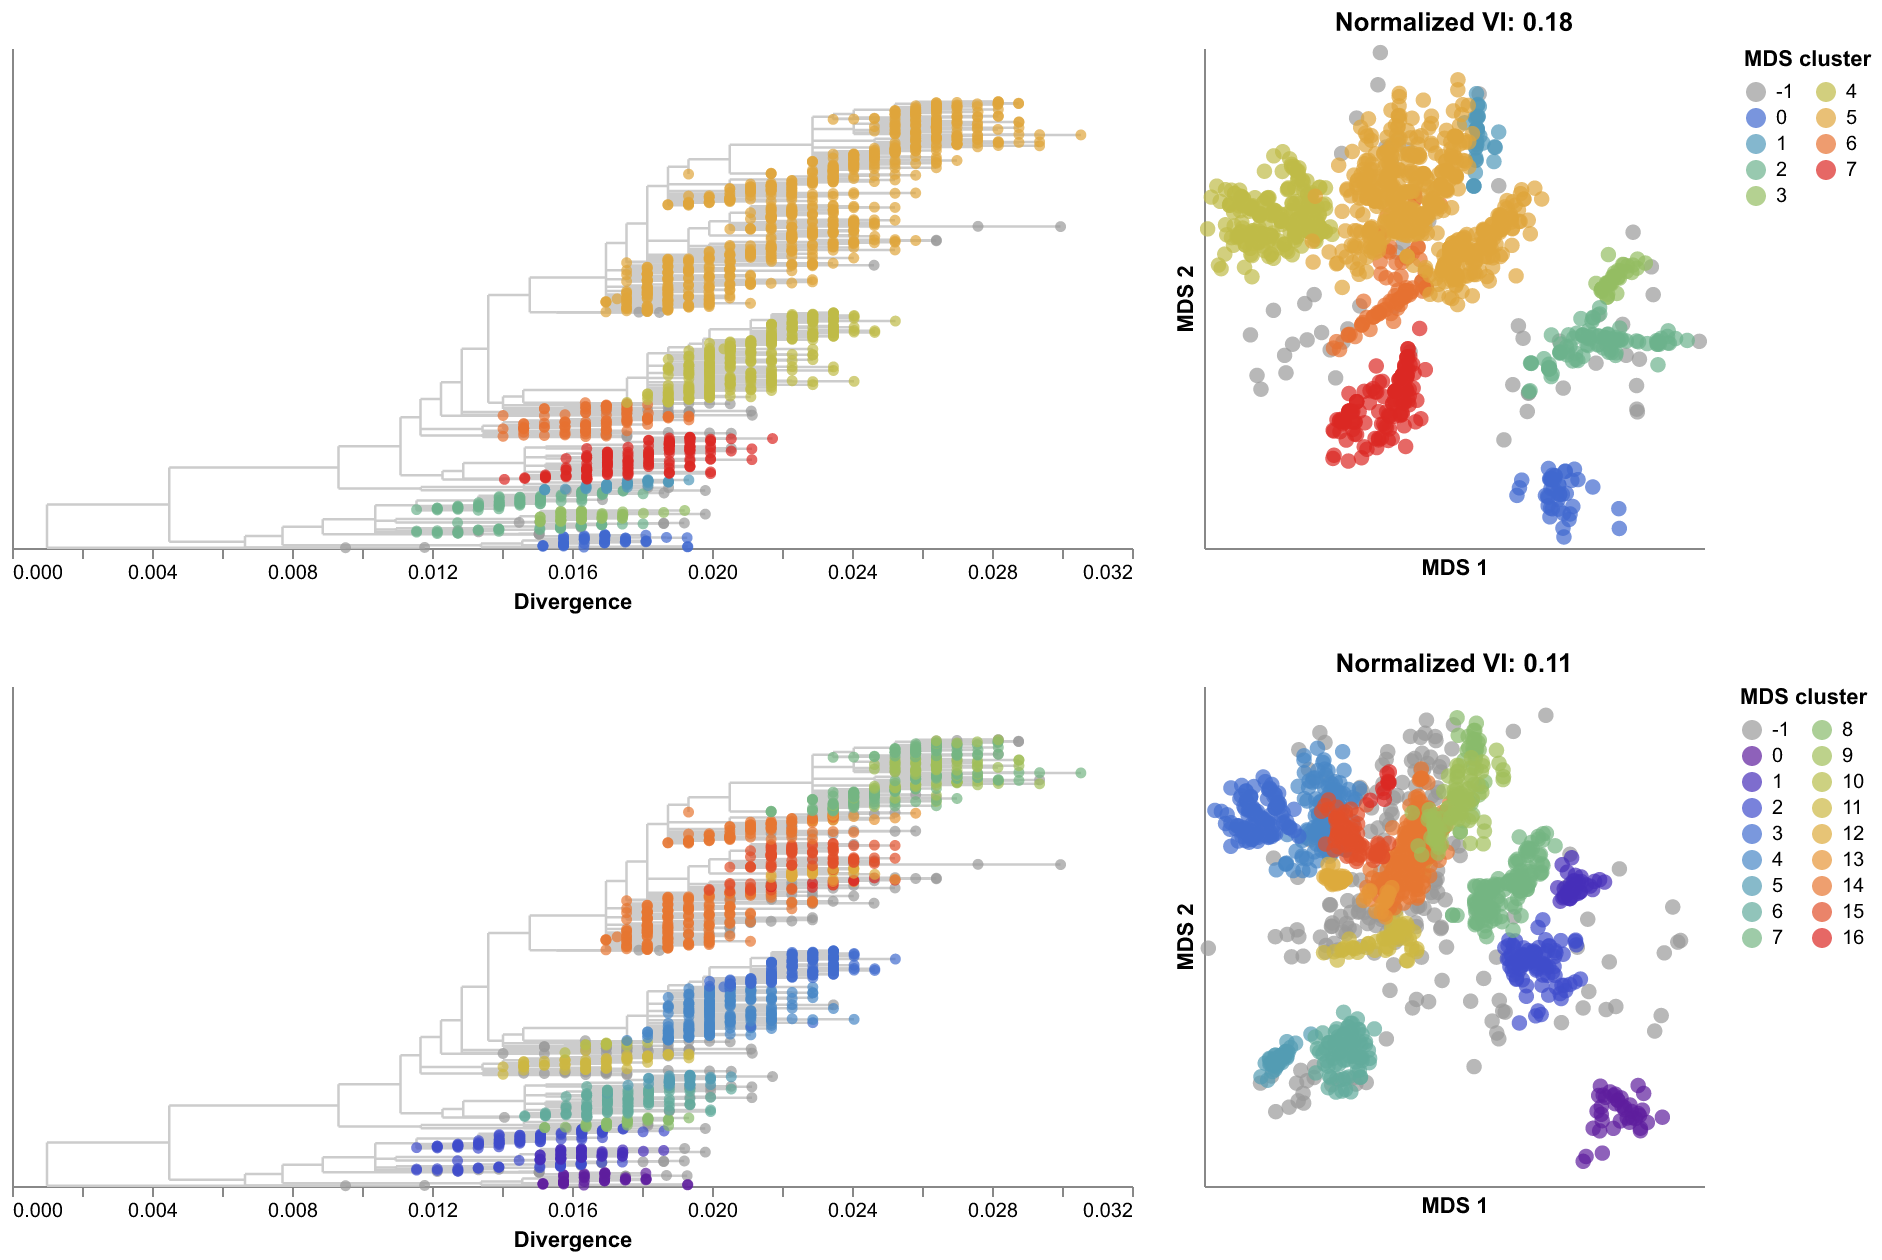
\includegraphics[width=\columnwidth]{figures/flu-2016-2018-ha-na-mds-by-cluster.png}
\caption*{{\bf S11 Fig. MDS embeddings for influenza H3N2 HA sequences only (top row) and HA/NA sequences combined (bottom row) showing the HA trees colored by clusters identified in each embedding (left) and the corresponding embeddings colored by cluster (right).}}
\end{figure}

\begin{figure}[!h]
% TODO: remove includegraphics commands in final submission; figures must be uploaded separately from the manuscript.
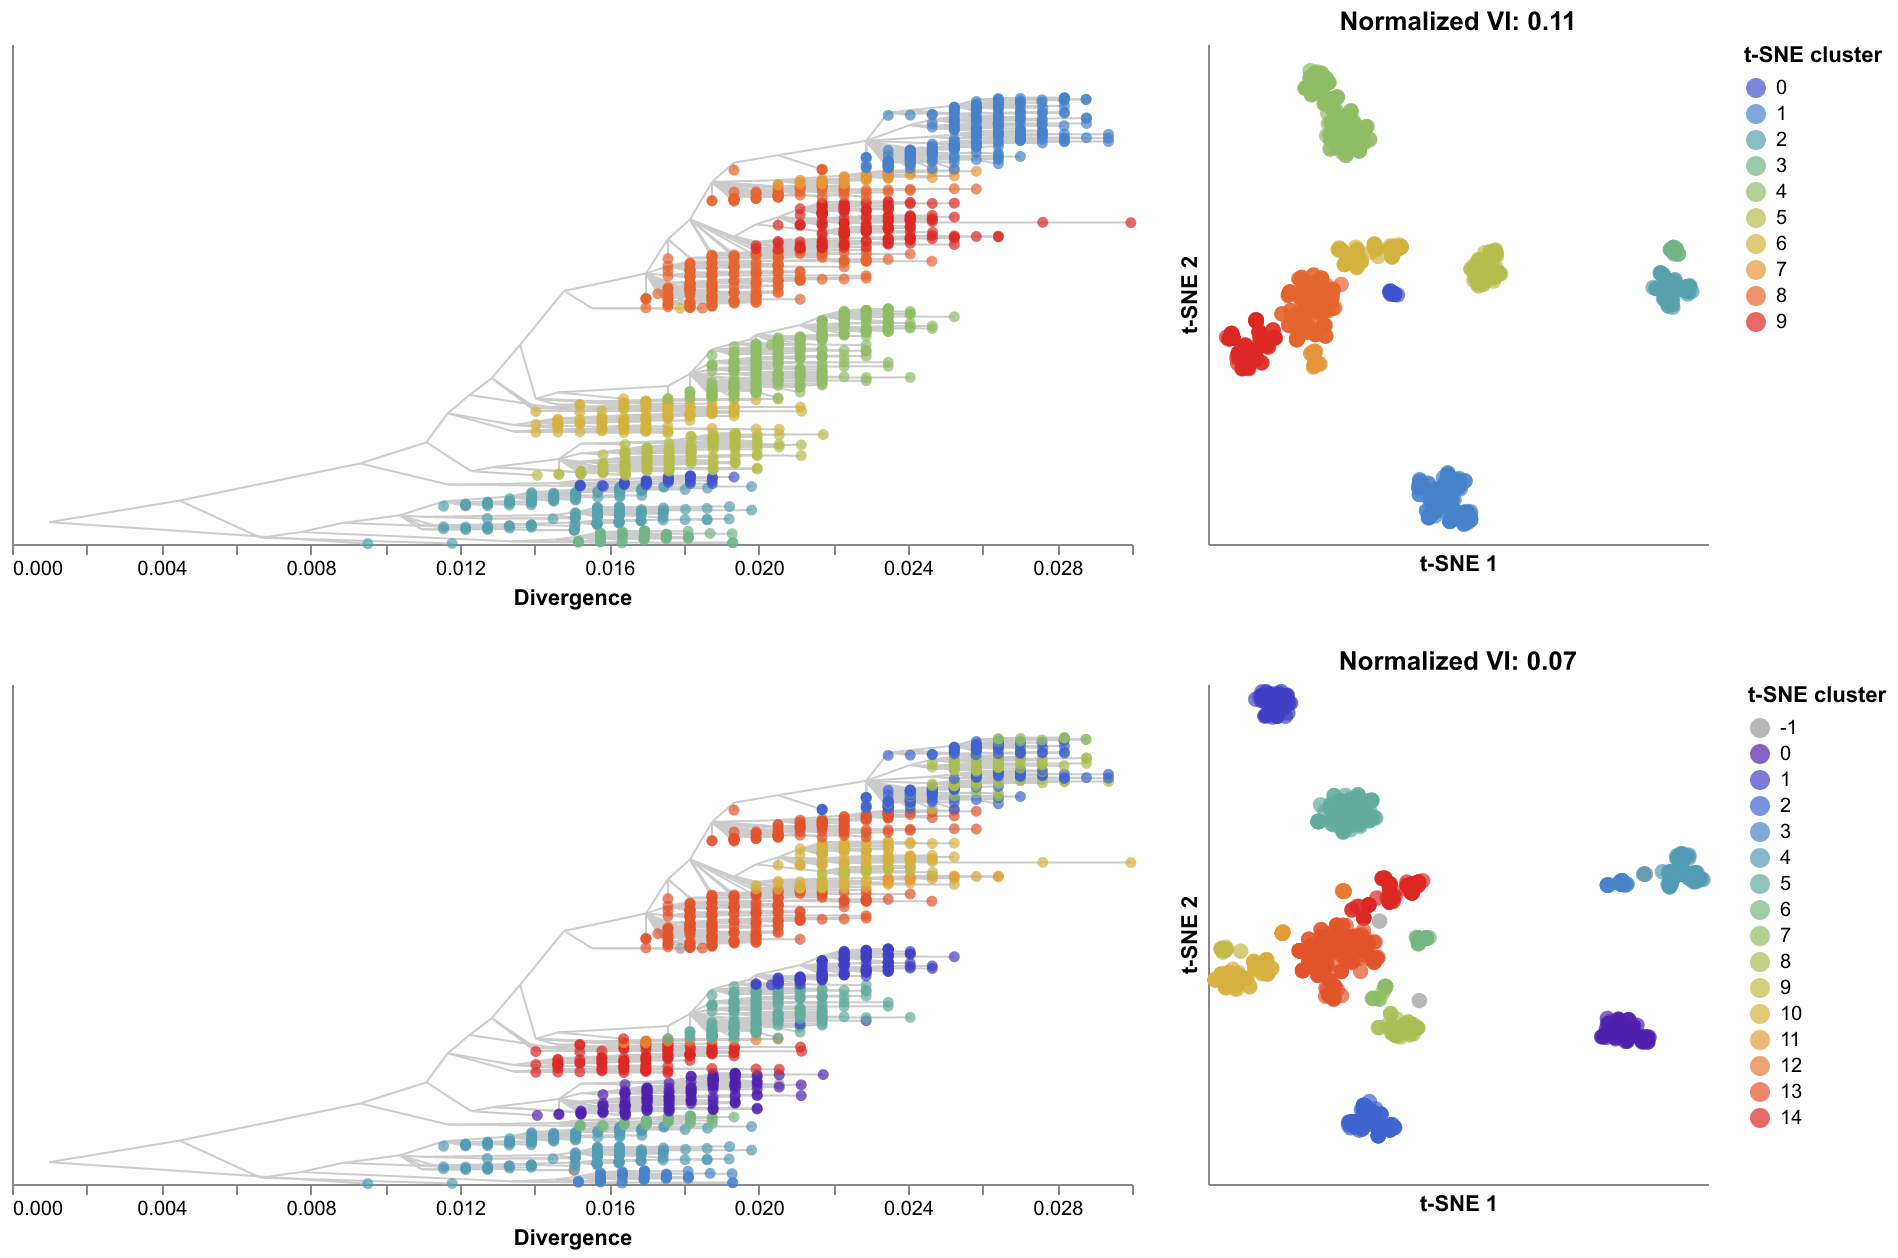
\includegraphics[width=\columnwidth]{figures/flu-2016-2018-ha-na-tsne-by-cluster.png}
\caption*{{\bf S12 Fig. t-SNE embeddings for influenza H3N2 HA sequences only (top row) and HA/NA sequences combined (bottom row) showing the HA trees colored by clusters identified in each embedding (left) and the corresponding embeddings colored by cluster (right).}}
\end{figure}

\begin{figure}[!h]
% TODO: remove includegraphics commands in final submission; figures must be uploaded separately from the manuscript.
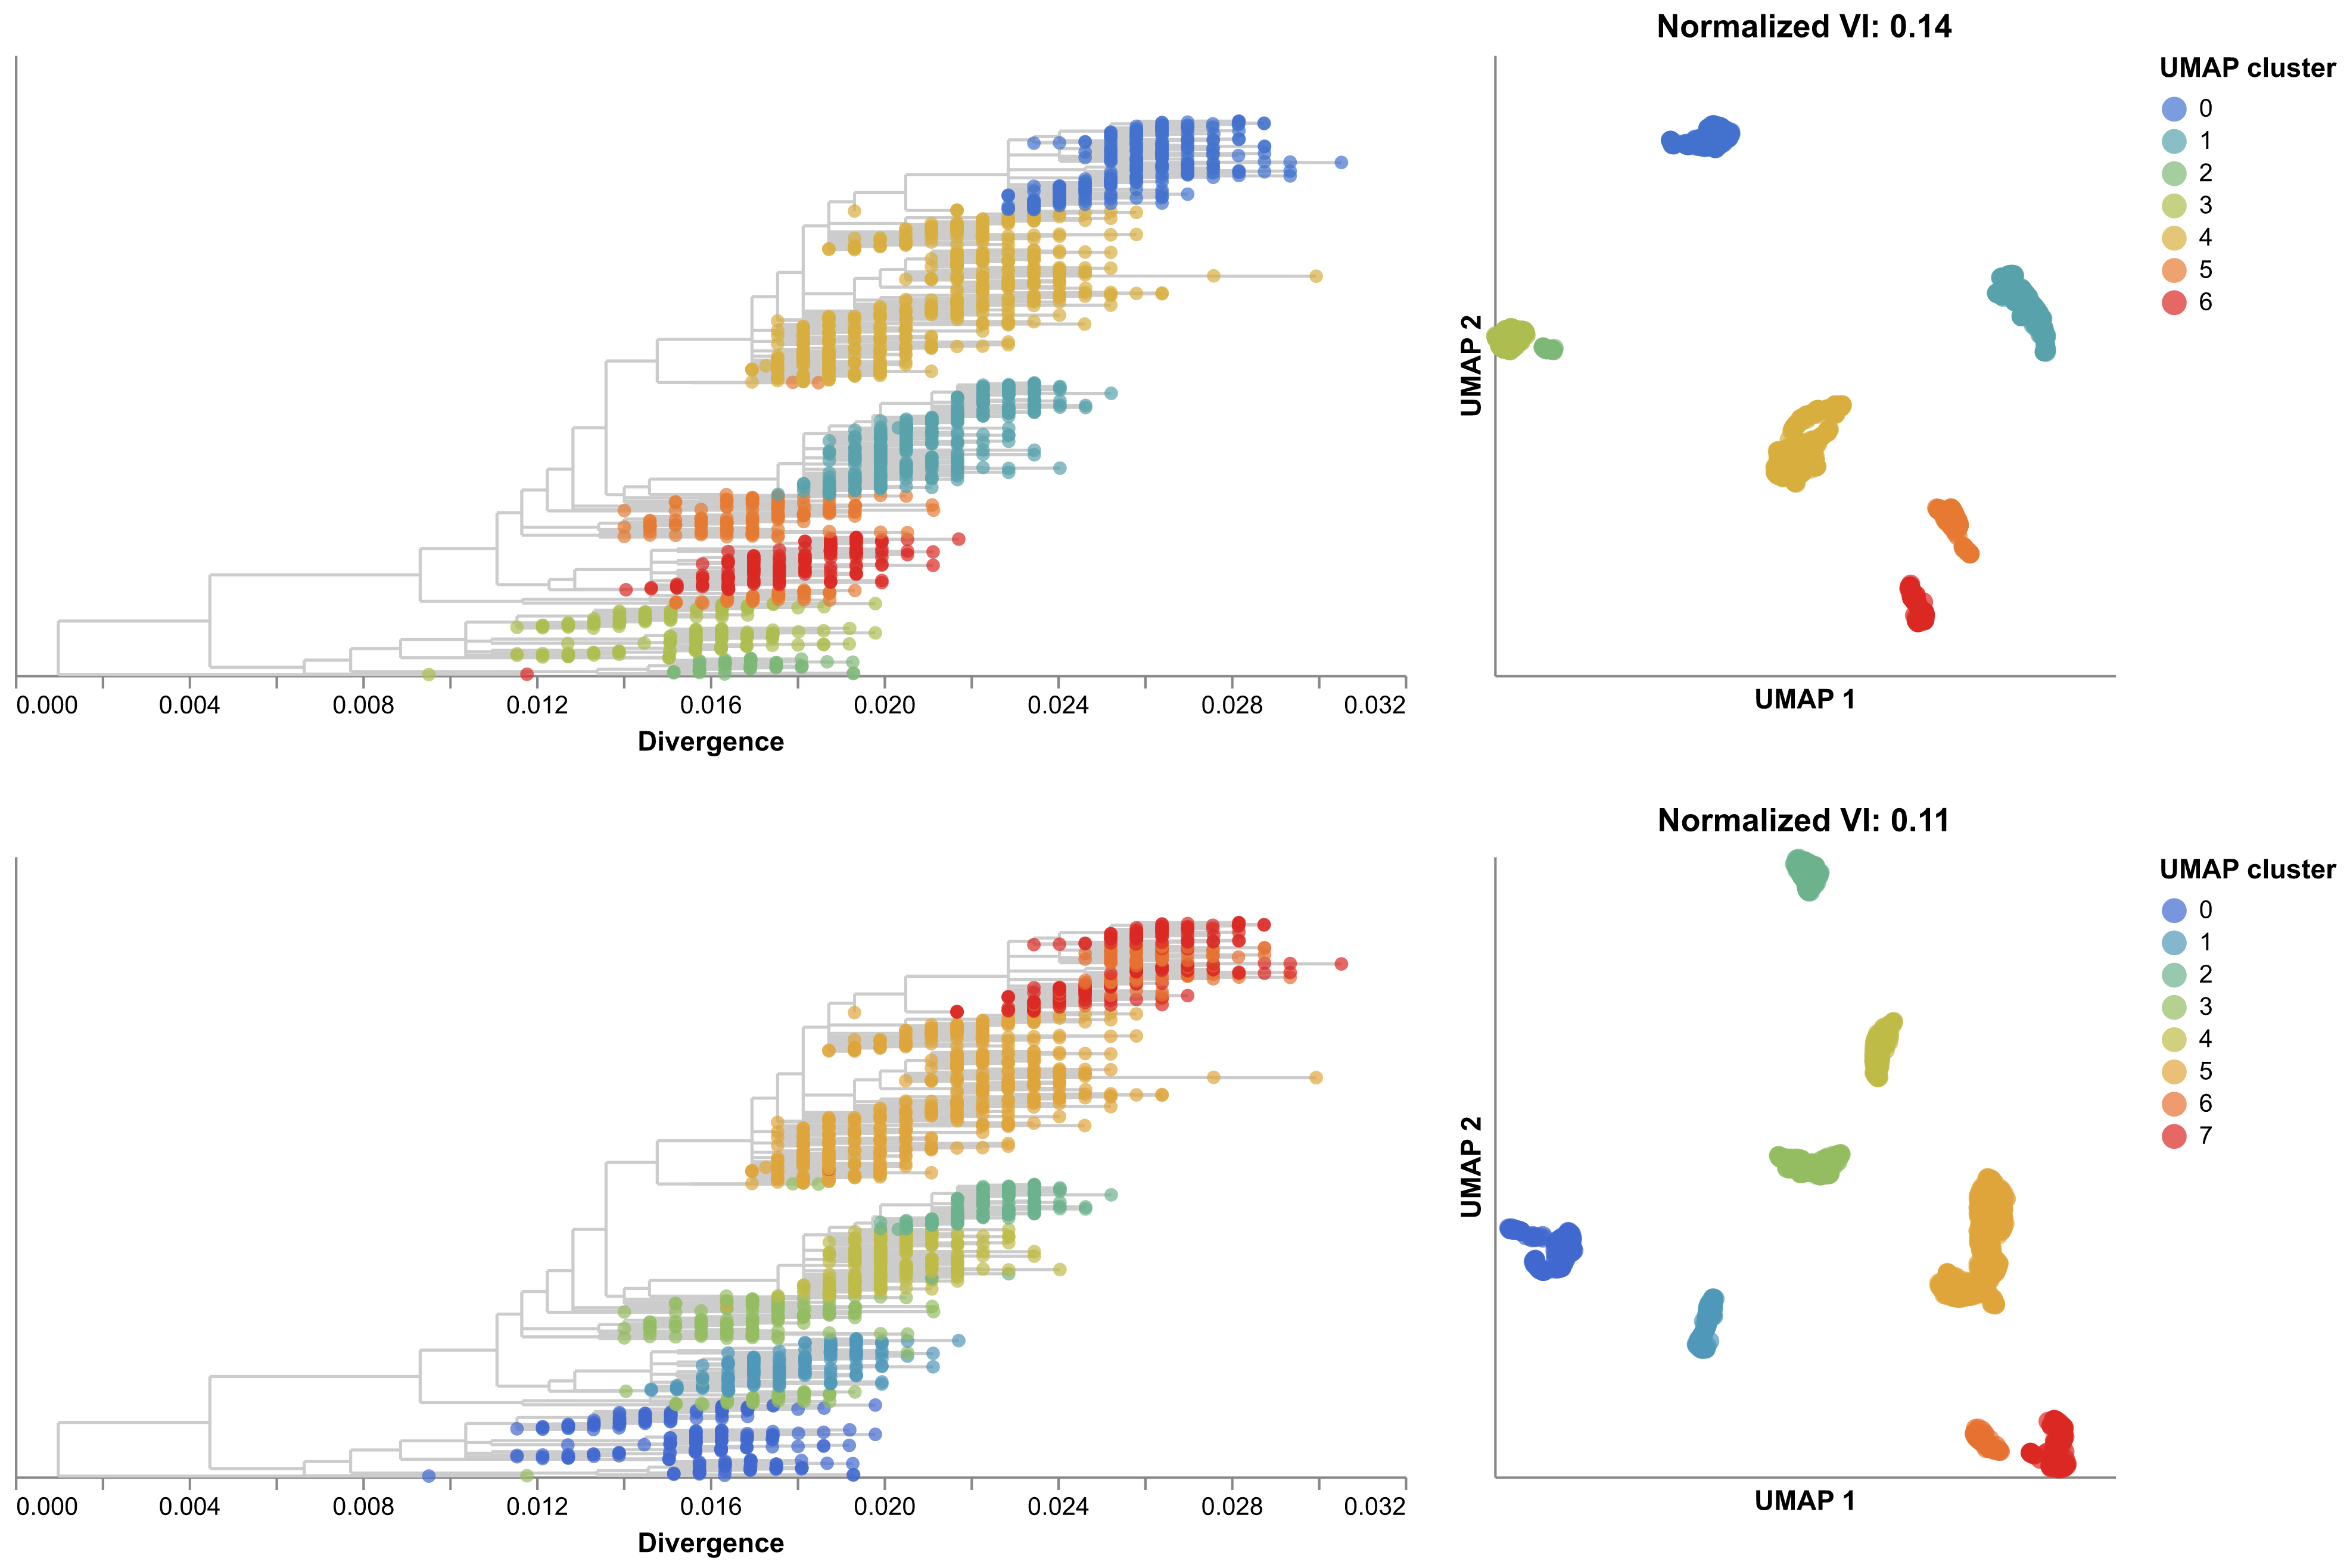
\includegraphics[width=\columnwidth]{figures/flu-2016-2018-ha-na-umap-by-cluster.png}
\caption*{{\bf S13 Fig. UMAP embeddings for influenza H3N2 HA sequences only (top row) and HA/NA sequences combined (bottom row) showing the HA trees colored by clusters identified in each embedding (left) and the corresponding embeddings colored by cluster (right).}}
\end{figure}

\begin{figure}[!h]
% TODO: remove includegraphics commands in final submission; figures must be uploaded separately from the manuscript.
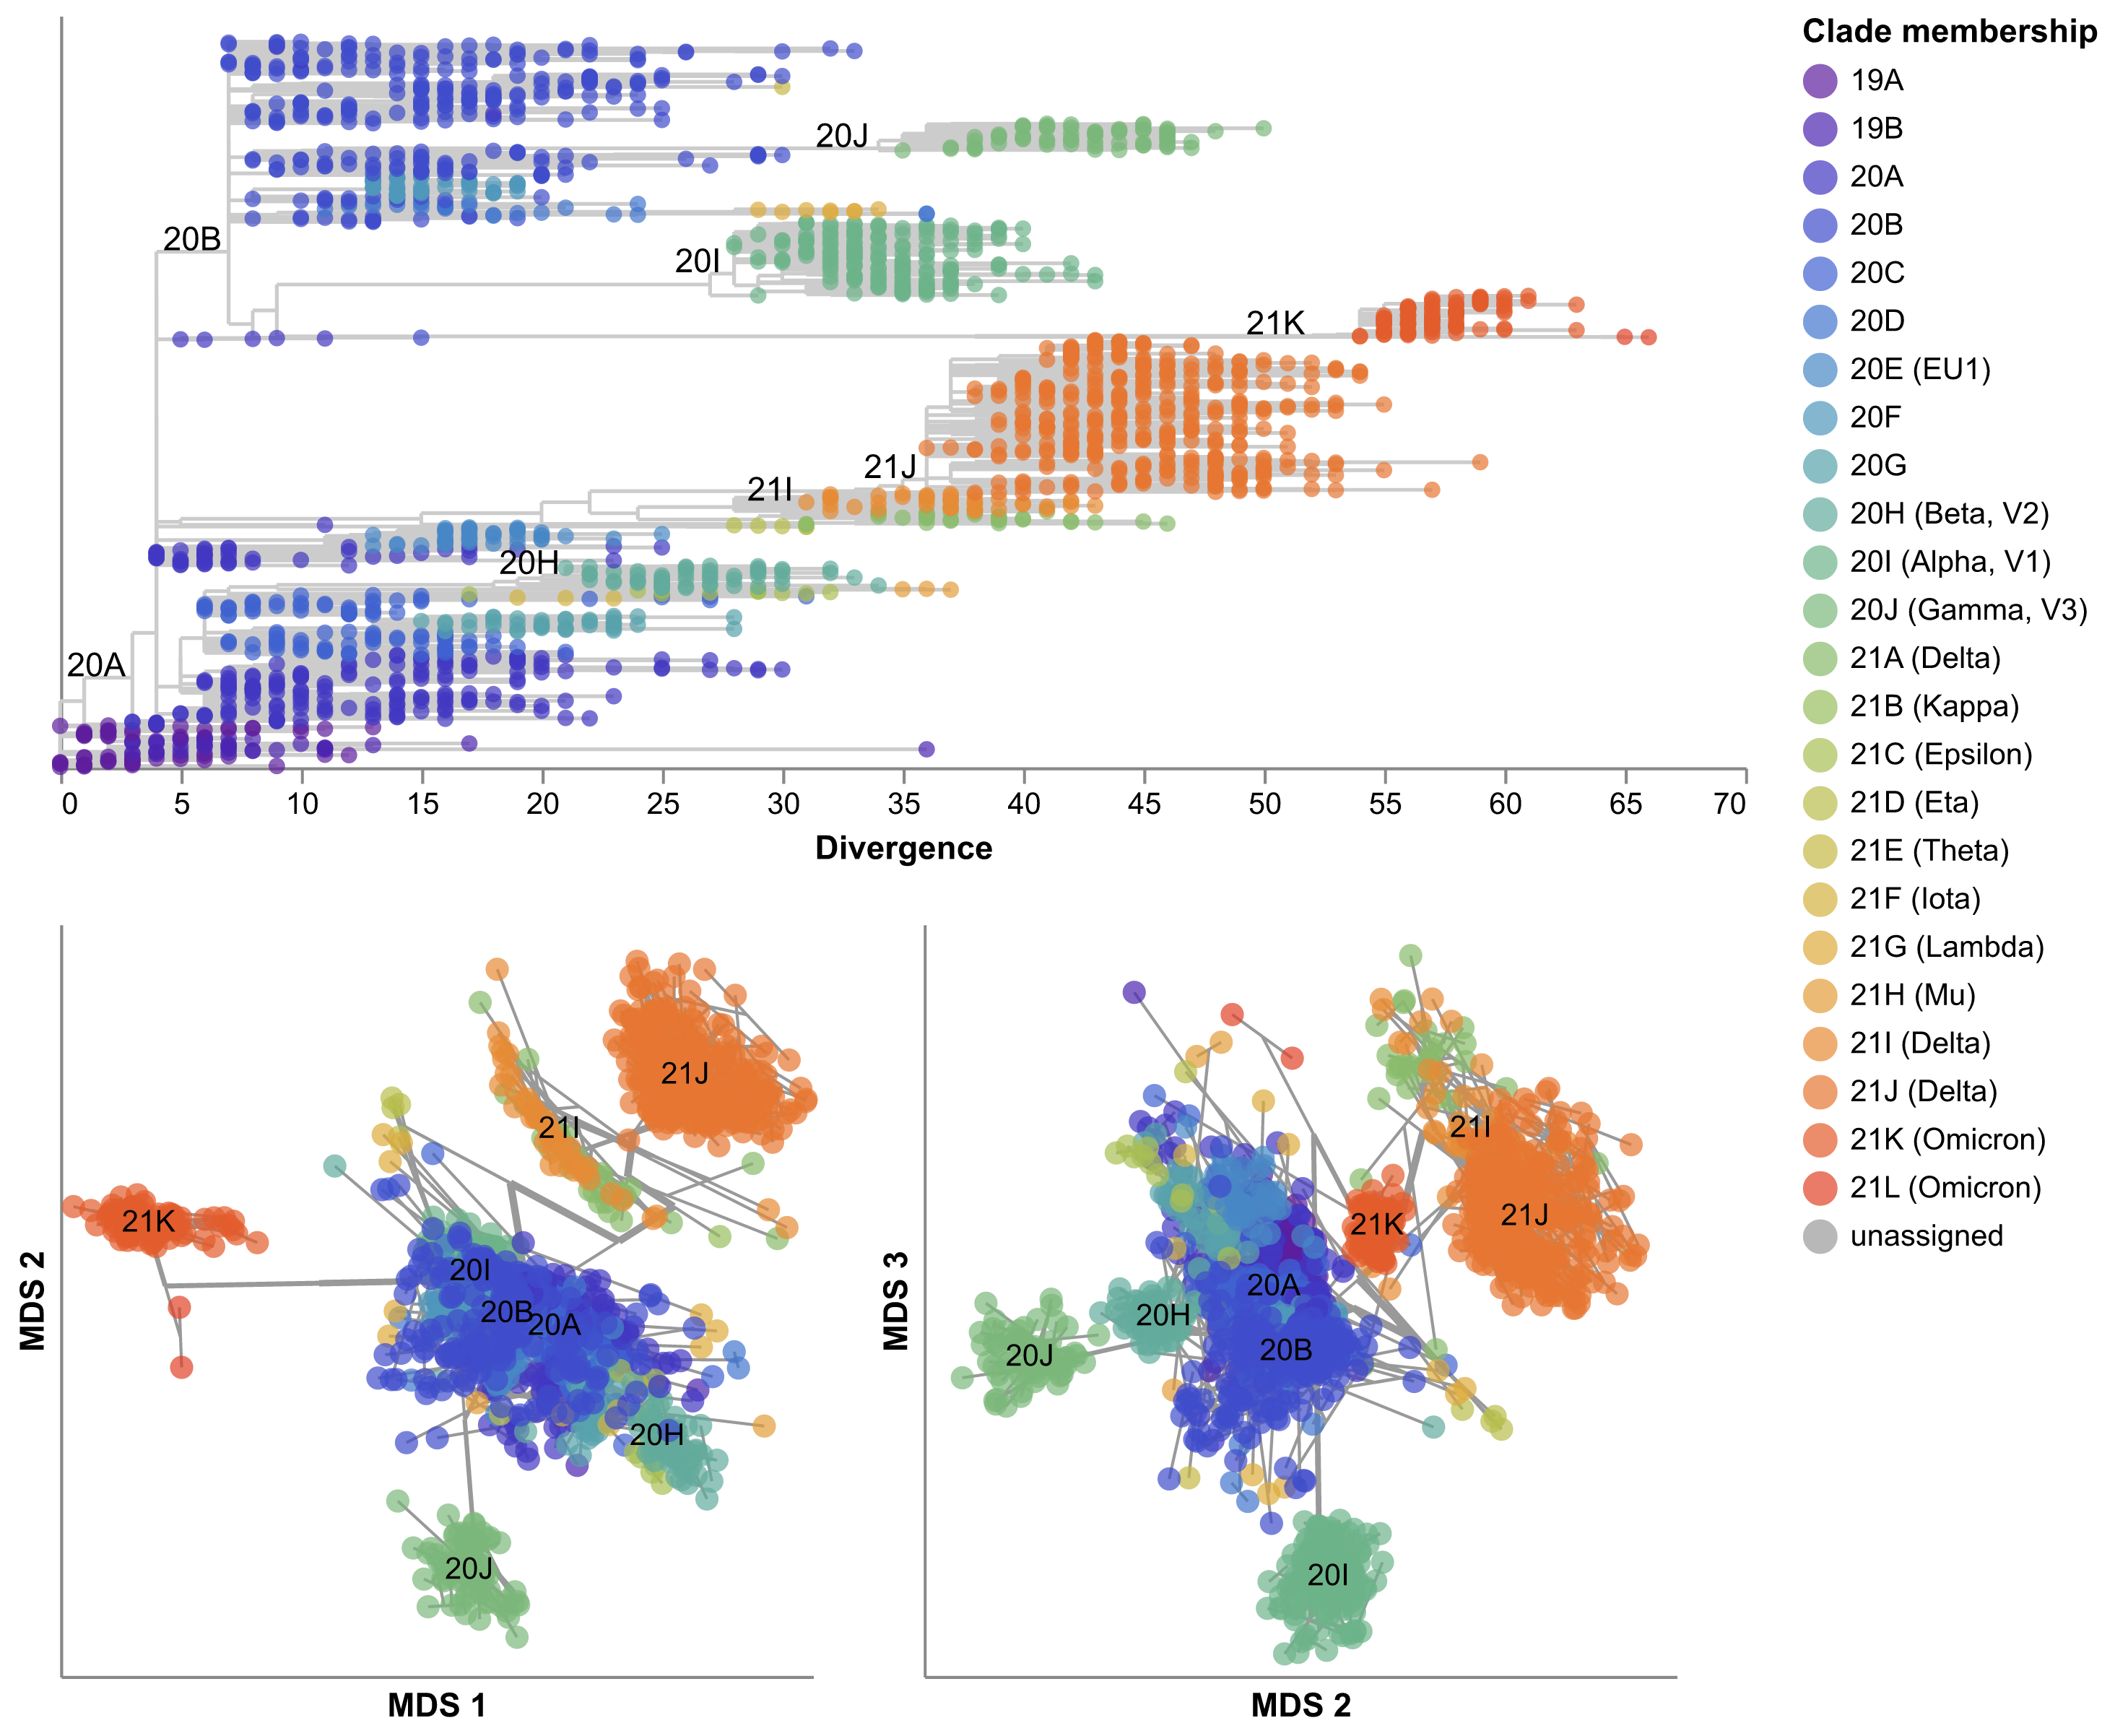
\includegraphics[width=\columnwidth]{figures/sarscov2-mds-by-Nextstrain_clade-clade.png}
\caption*{{\bf S14 Fig. MDS embeddings for early SARS-CoV-2 sequences showing all three components.}
  Line segments in each embedding reflect phylogenetic relationships with internal node positions calculated from the mean positions of their immediate descendants in each dimension (see Methods).
  Line thickness scales by the square root of the number of leaves descending from a given node in the phylogeny.}
\end{figure}

\begin{figure}[!h]
% TODO: remove includegraphics commands in final submission; figures must be uploaded separately from the manuscript.
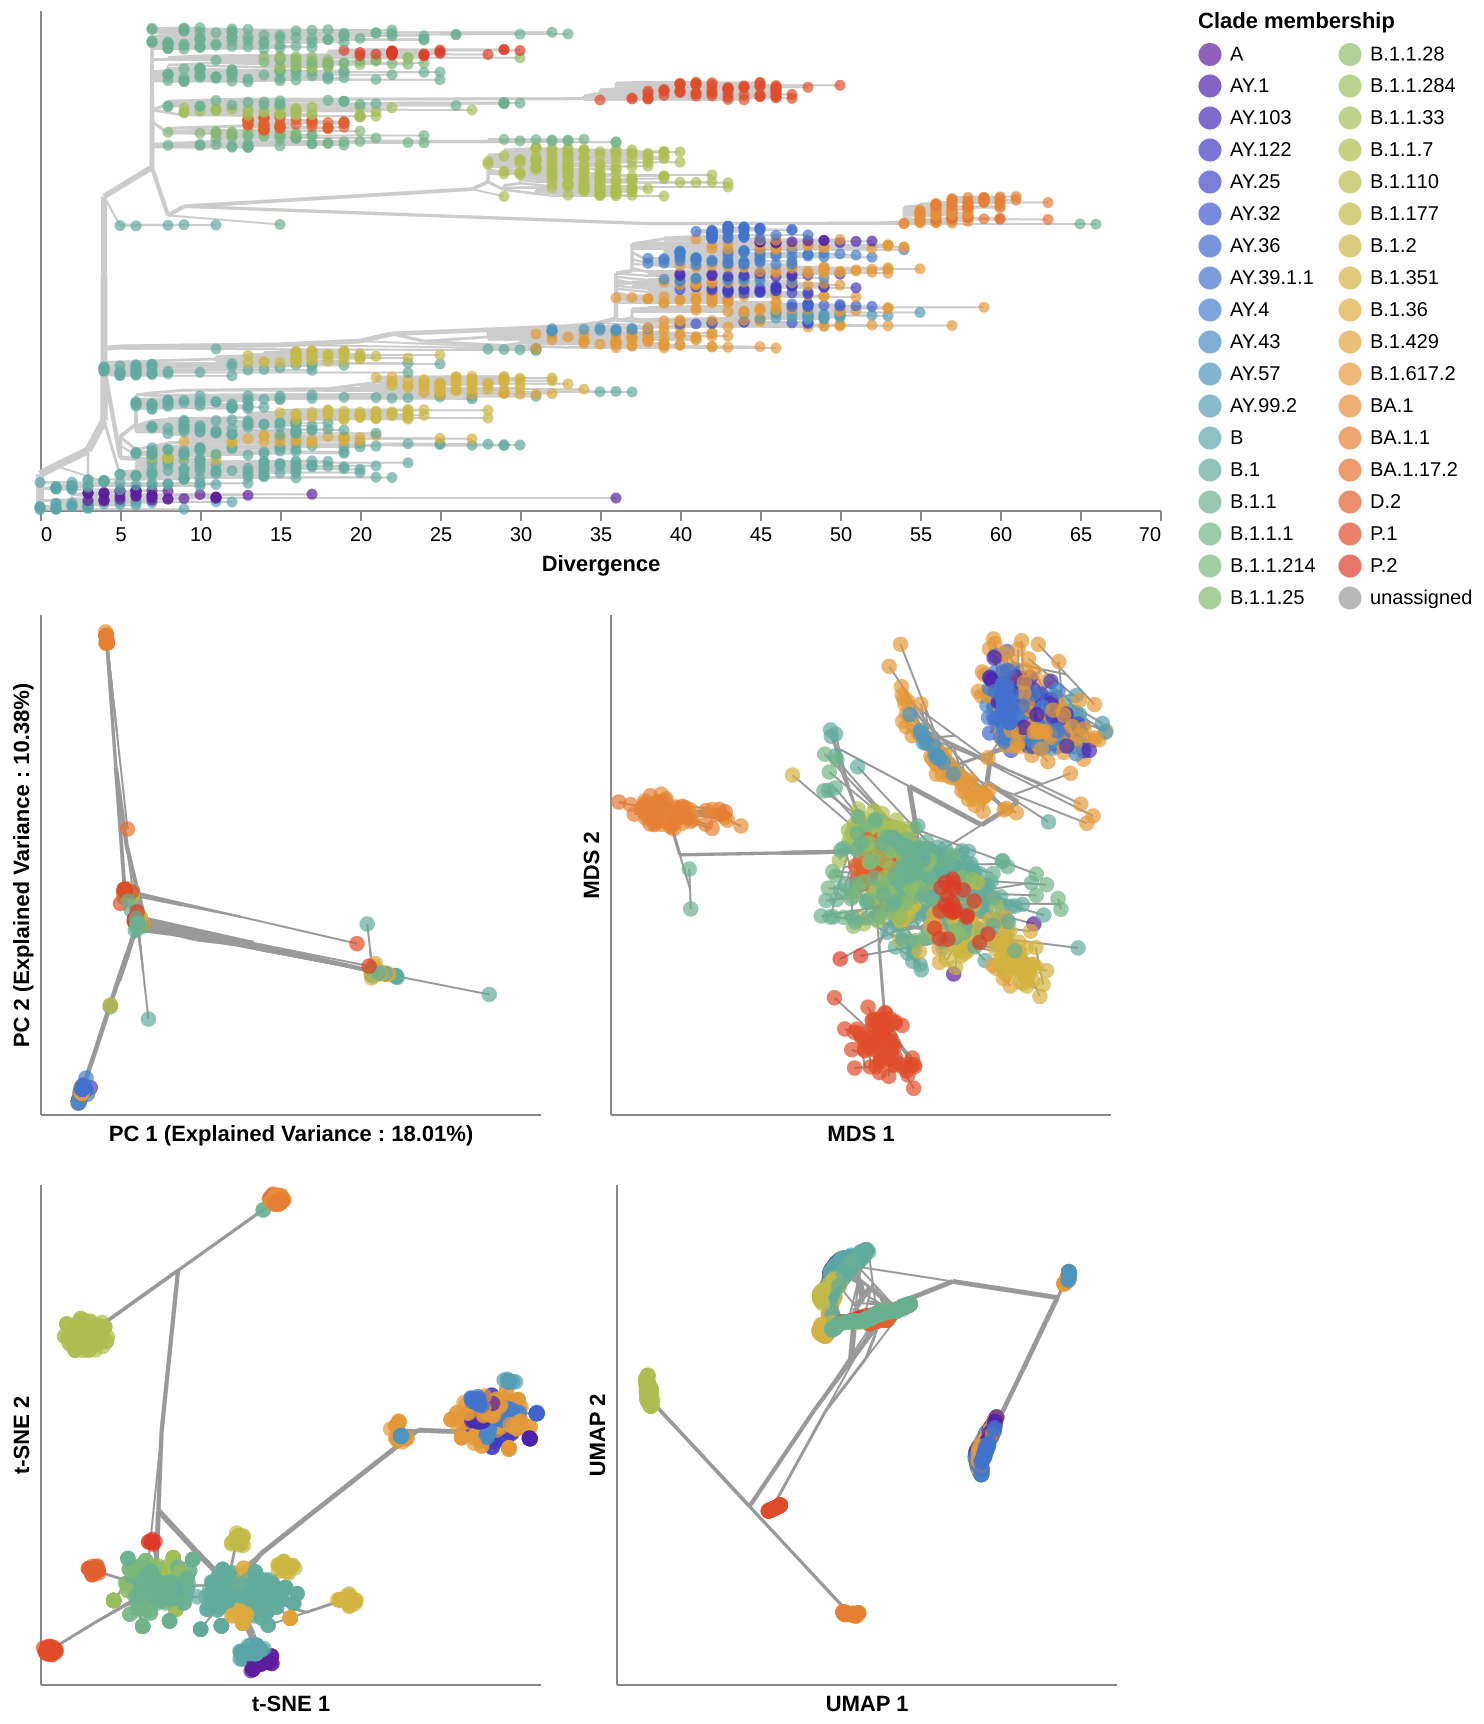
\includegraphics[width=\columnwidth]{figures/sarscov2-embeddings-by-Nextclade_pango_collapsed-clade.png}
\caption*{{\bf S15 Fig. Phylogeny of early (2020--2022) SARS-CoV-2 sequences plotted by number of nucleotide substitutions from the most recent common ancestor on the x-axis (top) and low-dimensional embeddings of the same sequences by PCA (middle left), MDS (middle right), t-SNE (bottom left), and UMAP (bottom right).}
  Tips in the tree and embeddings are colored by their Pango lineage assignment.
  Line segments in each embedding reflect phylogenetic relationships with internal node positions calculated from the mean positions of their immediate descendants in each dimension (see Methods).
  Line thickness scales by the square root of the number of leaves descending from a given node in the phylogeny.
}
\end{figure}

\begin{figure}[!h]
% TODO: remove includegraphics commands in final submission; figures must be uploaded separately from the manuscript.
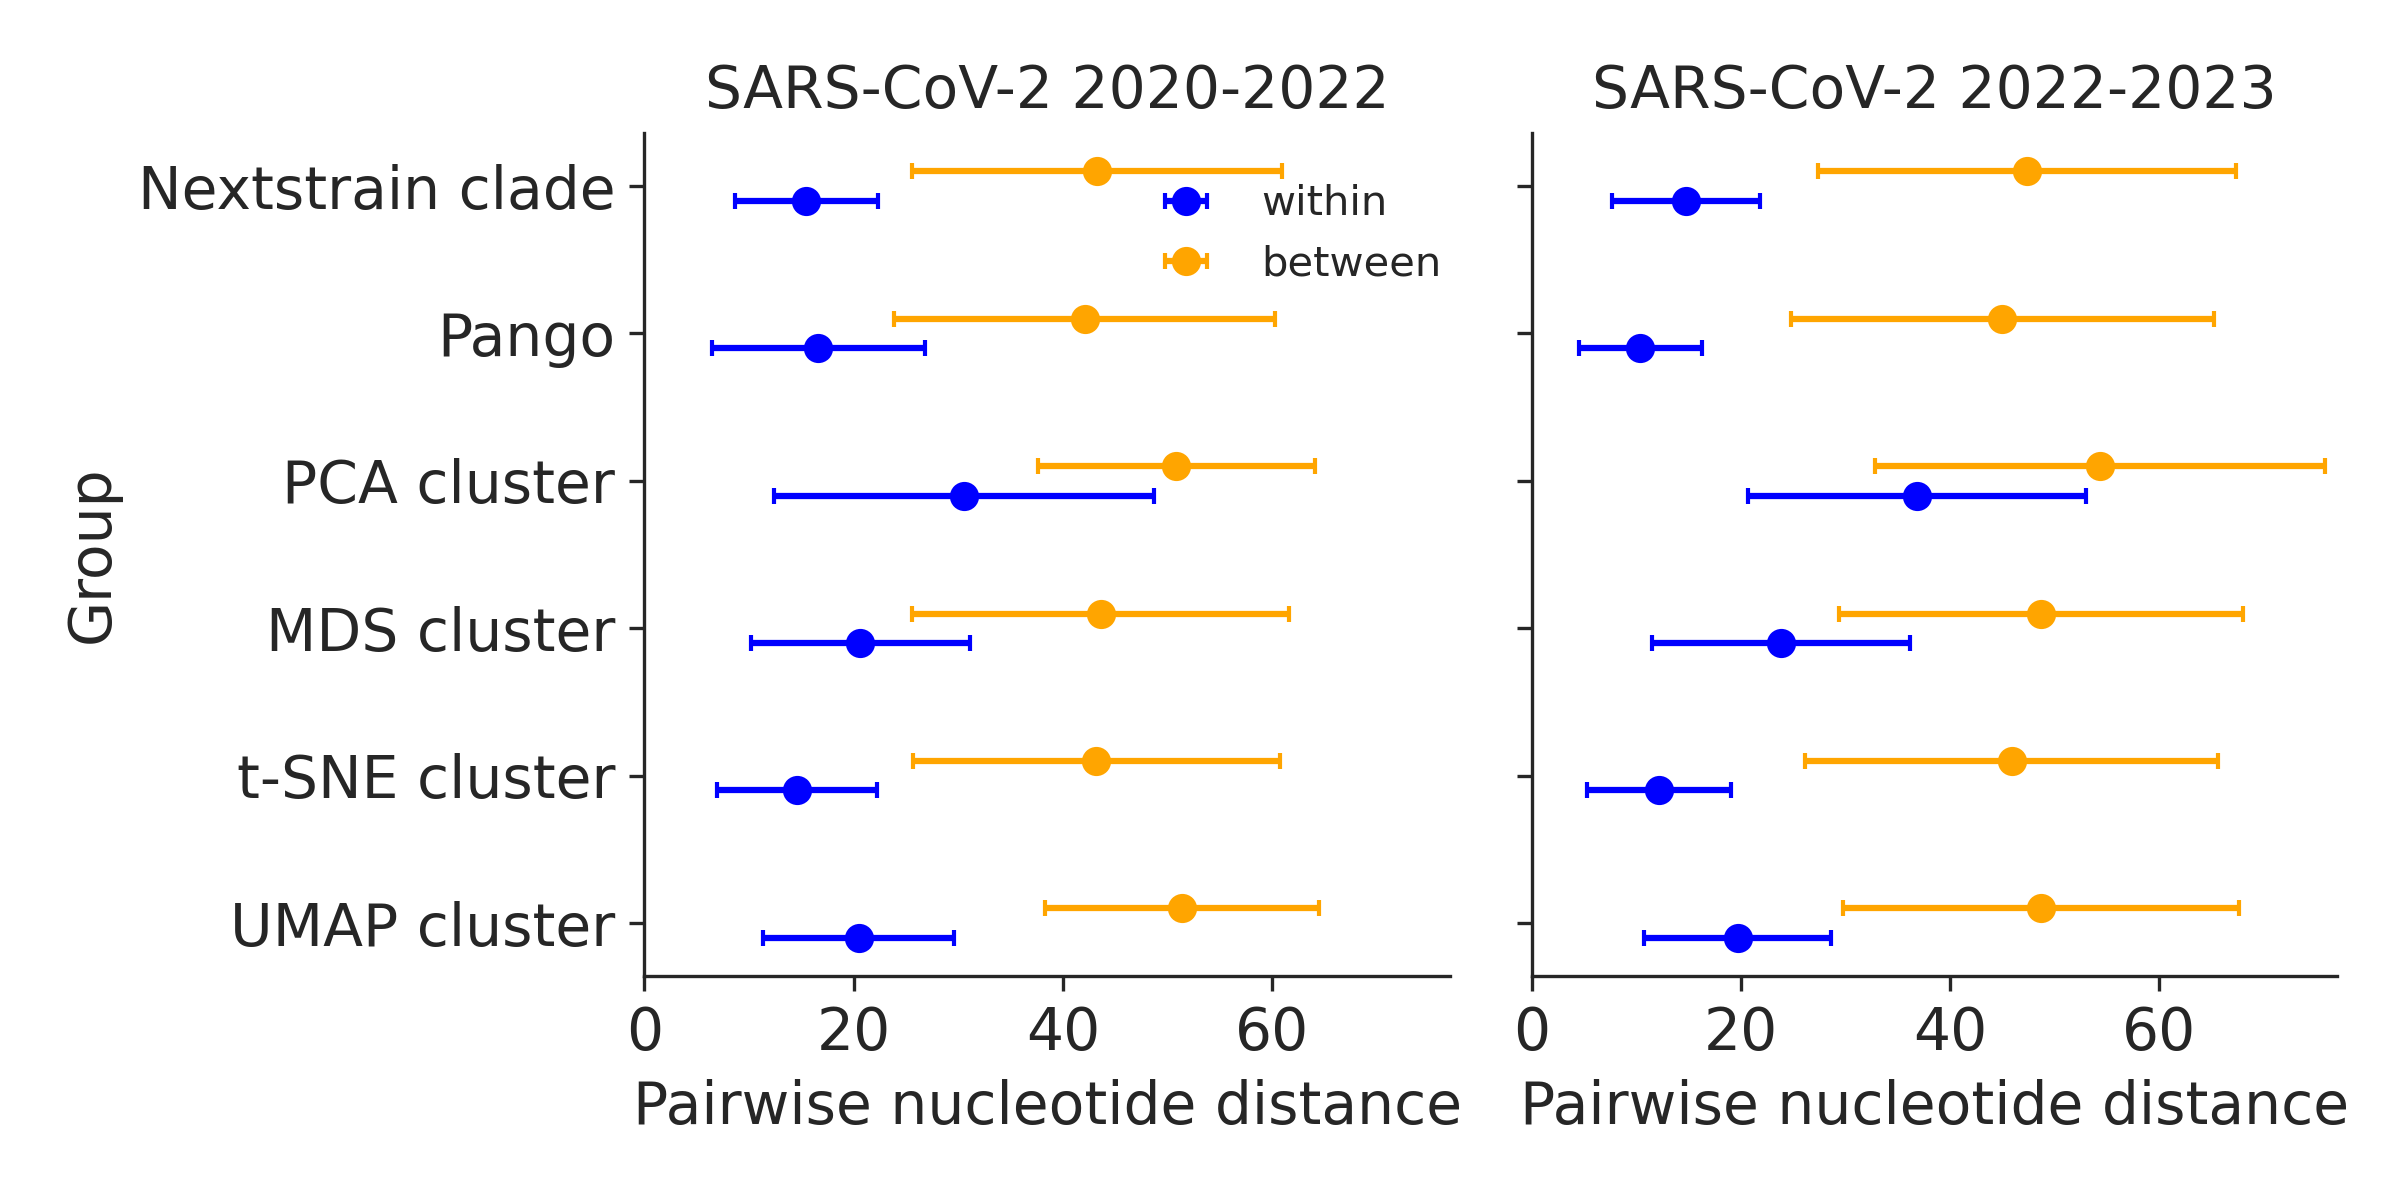
\includegraphics[width=\columnwidth]{figures/within_between_sars.png}
\caption*{{\bf S16 Fig. Pairwise nucleotide distances for early (2020-2022) and late (2022-2023) SARS-CoV-2 sequences within and between genetic groups defined by Nextstrain clades, Pango lineages, and clusters from PCA, MDS, t-SNE, and UMAP embeddings.}}
\end{figure}

\begin{figure}[!h]
% TODO: remove includegraphics commands in final submission; figures must be uploaded separately from the manuscript.
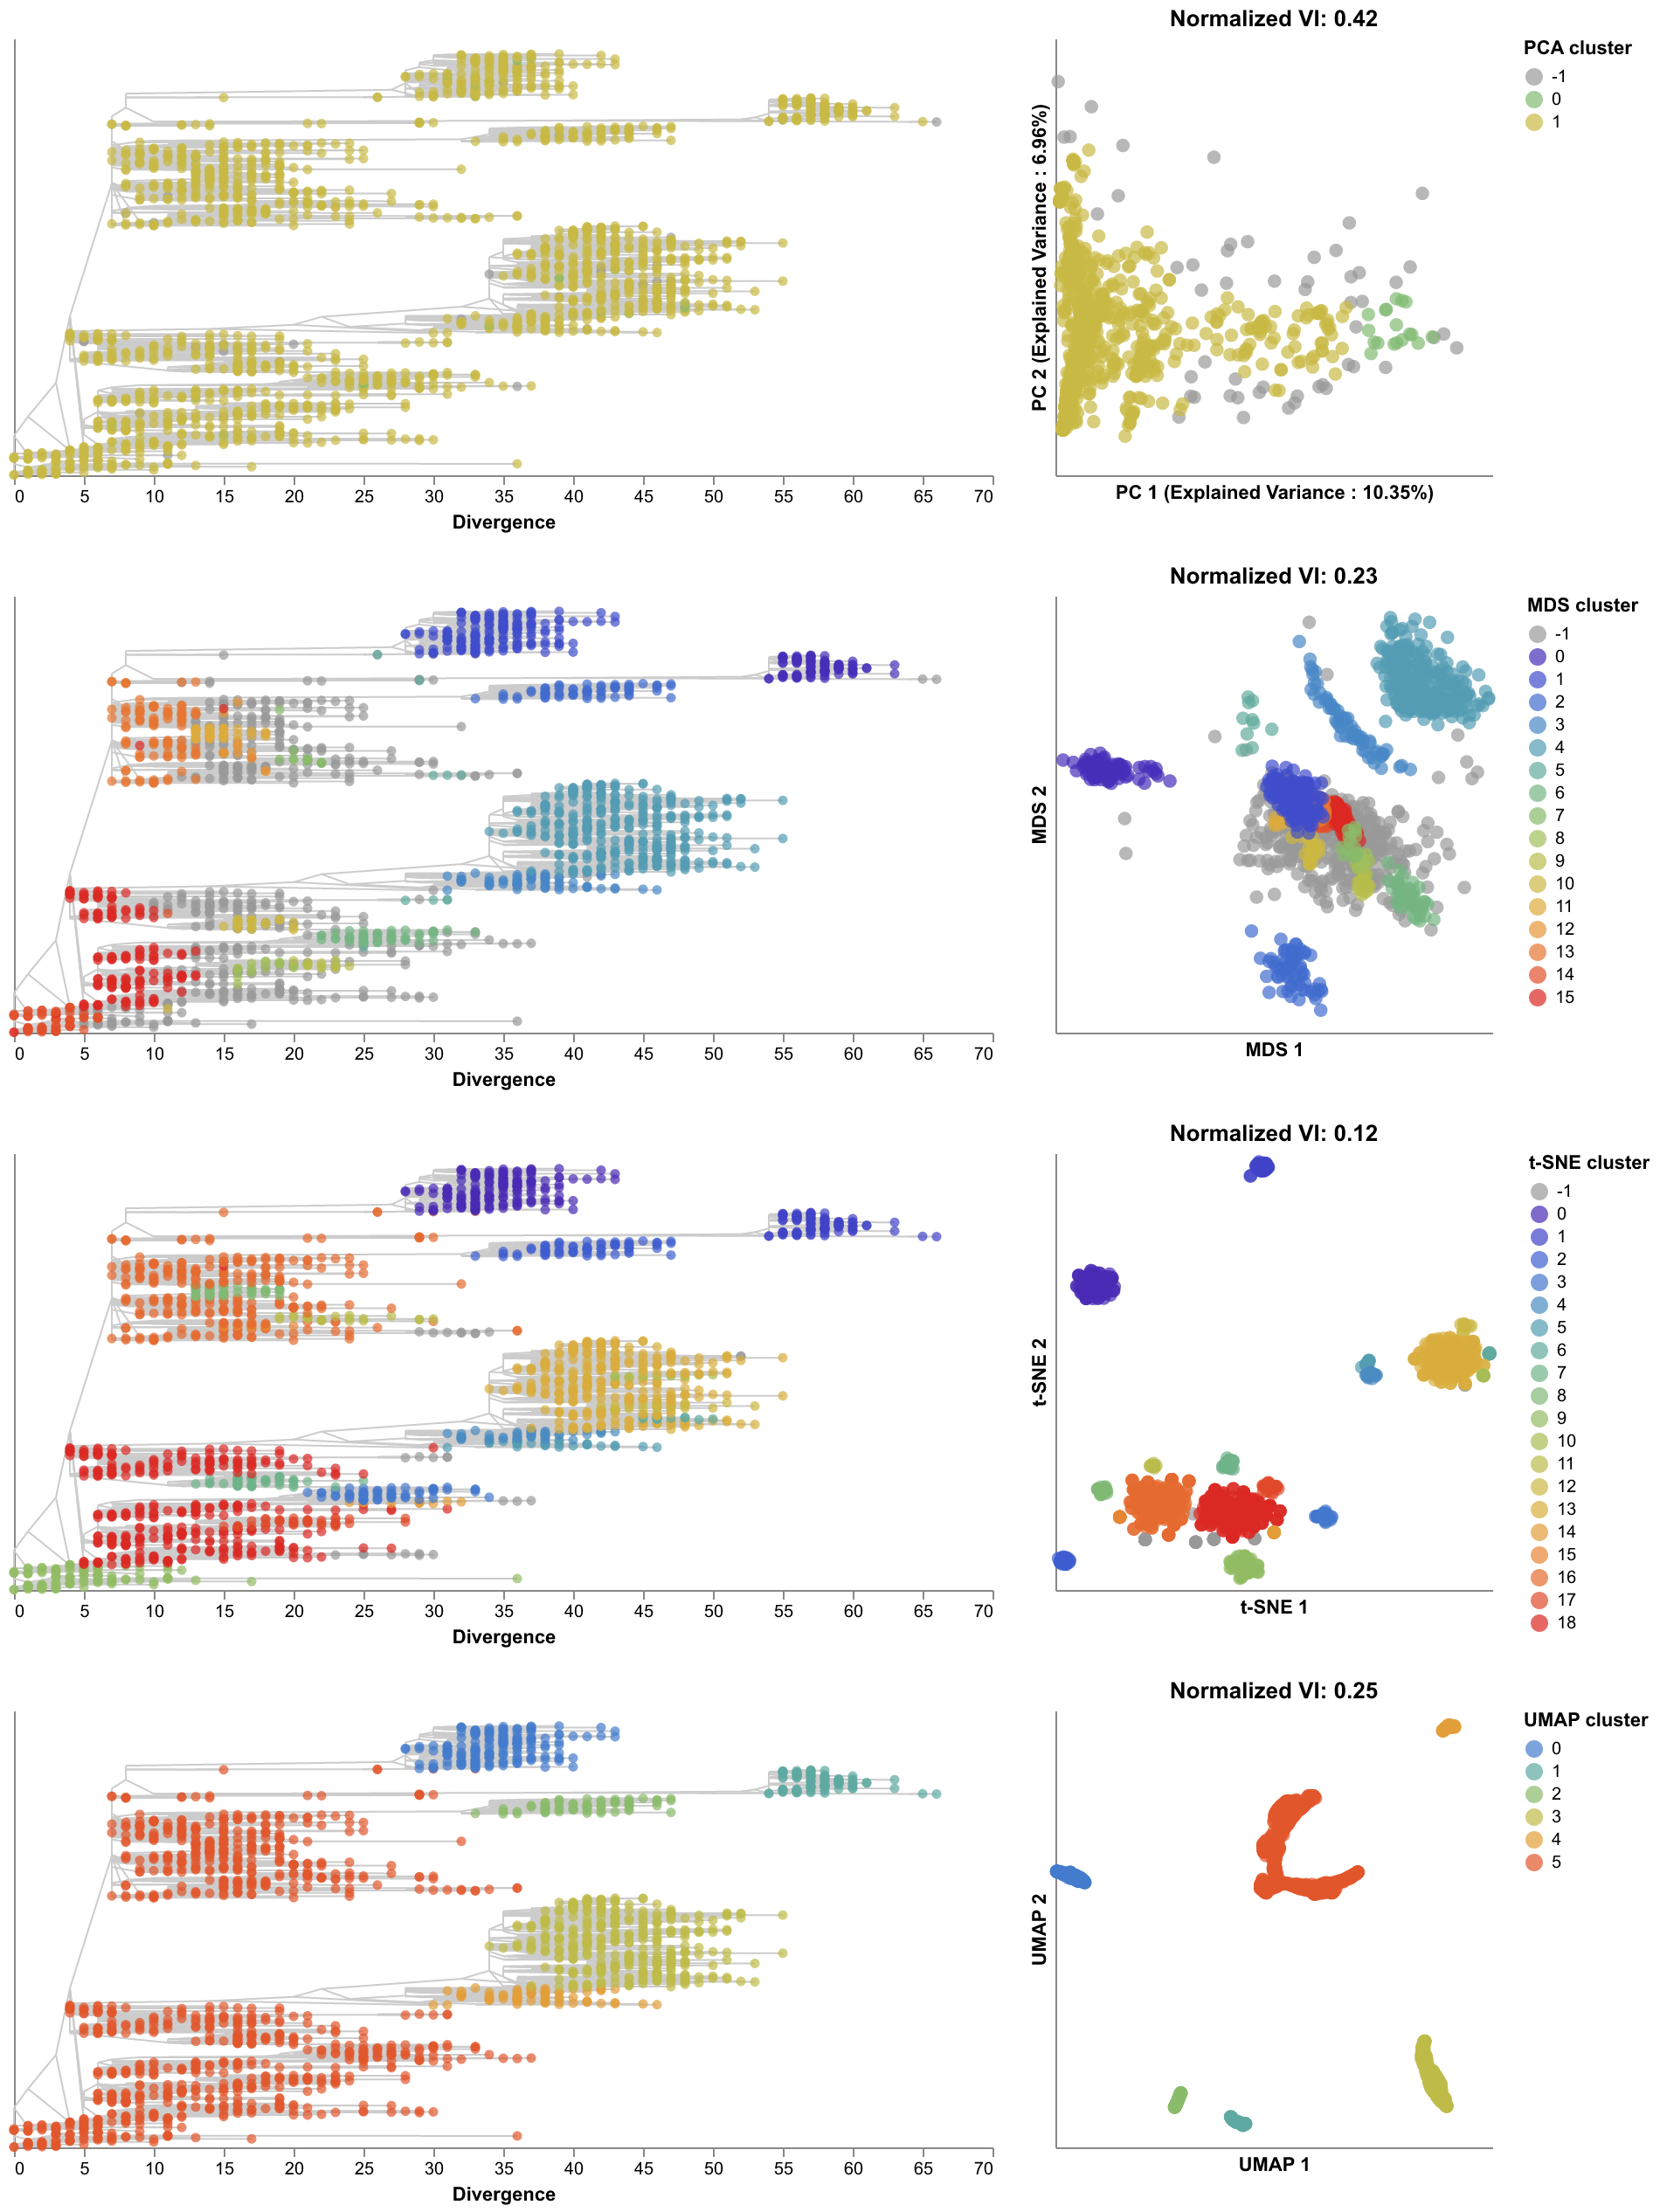
\includegraphics[width=\columnwidth]{figures/sarscov2-embeddings-by-cluster-vs-Nextclade_pango_collapsed.png}
\caption*{{\bf S17 Fig. Phylogenetic trees (left) and embeddings (right) of early (2020--2022) SARS-CoV-2 sequences colored by HDBSCAN cluster.}
  Normalized VI values per embedding reflect the distance between clusters and known genetic groups (Pango lineages).
  Line segments in each embedding reflect phylogenetic relationships with internal node positions calculated from the mean positions of their immediate descendants in each dimension (see Methods).
  Line thickness scales by the square root of the number of leaves descending from a given node in the phylogeny.
}
\end{figure}

\begin{figure}[!h]
% TODO: remove includegraphics commands in final submission; figures must be uploaded separately from the manuscript.
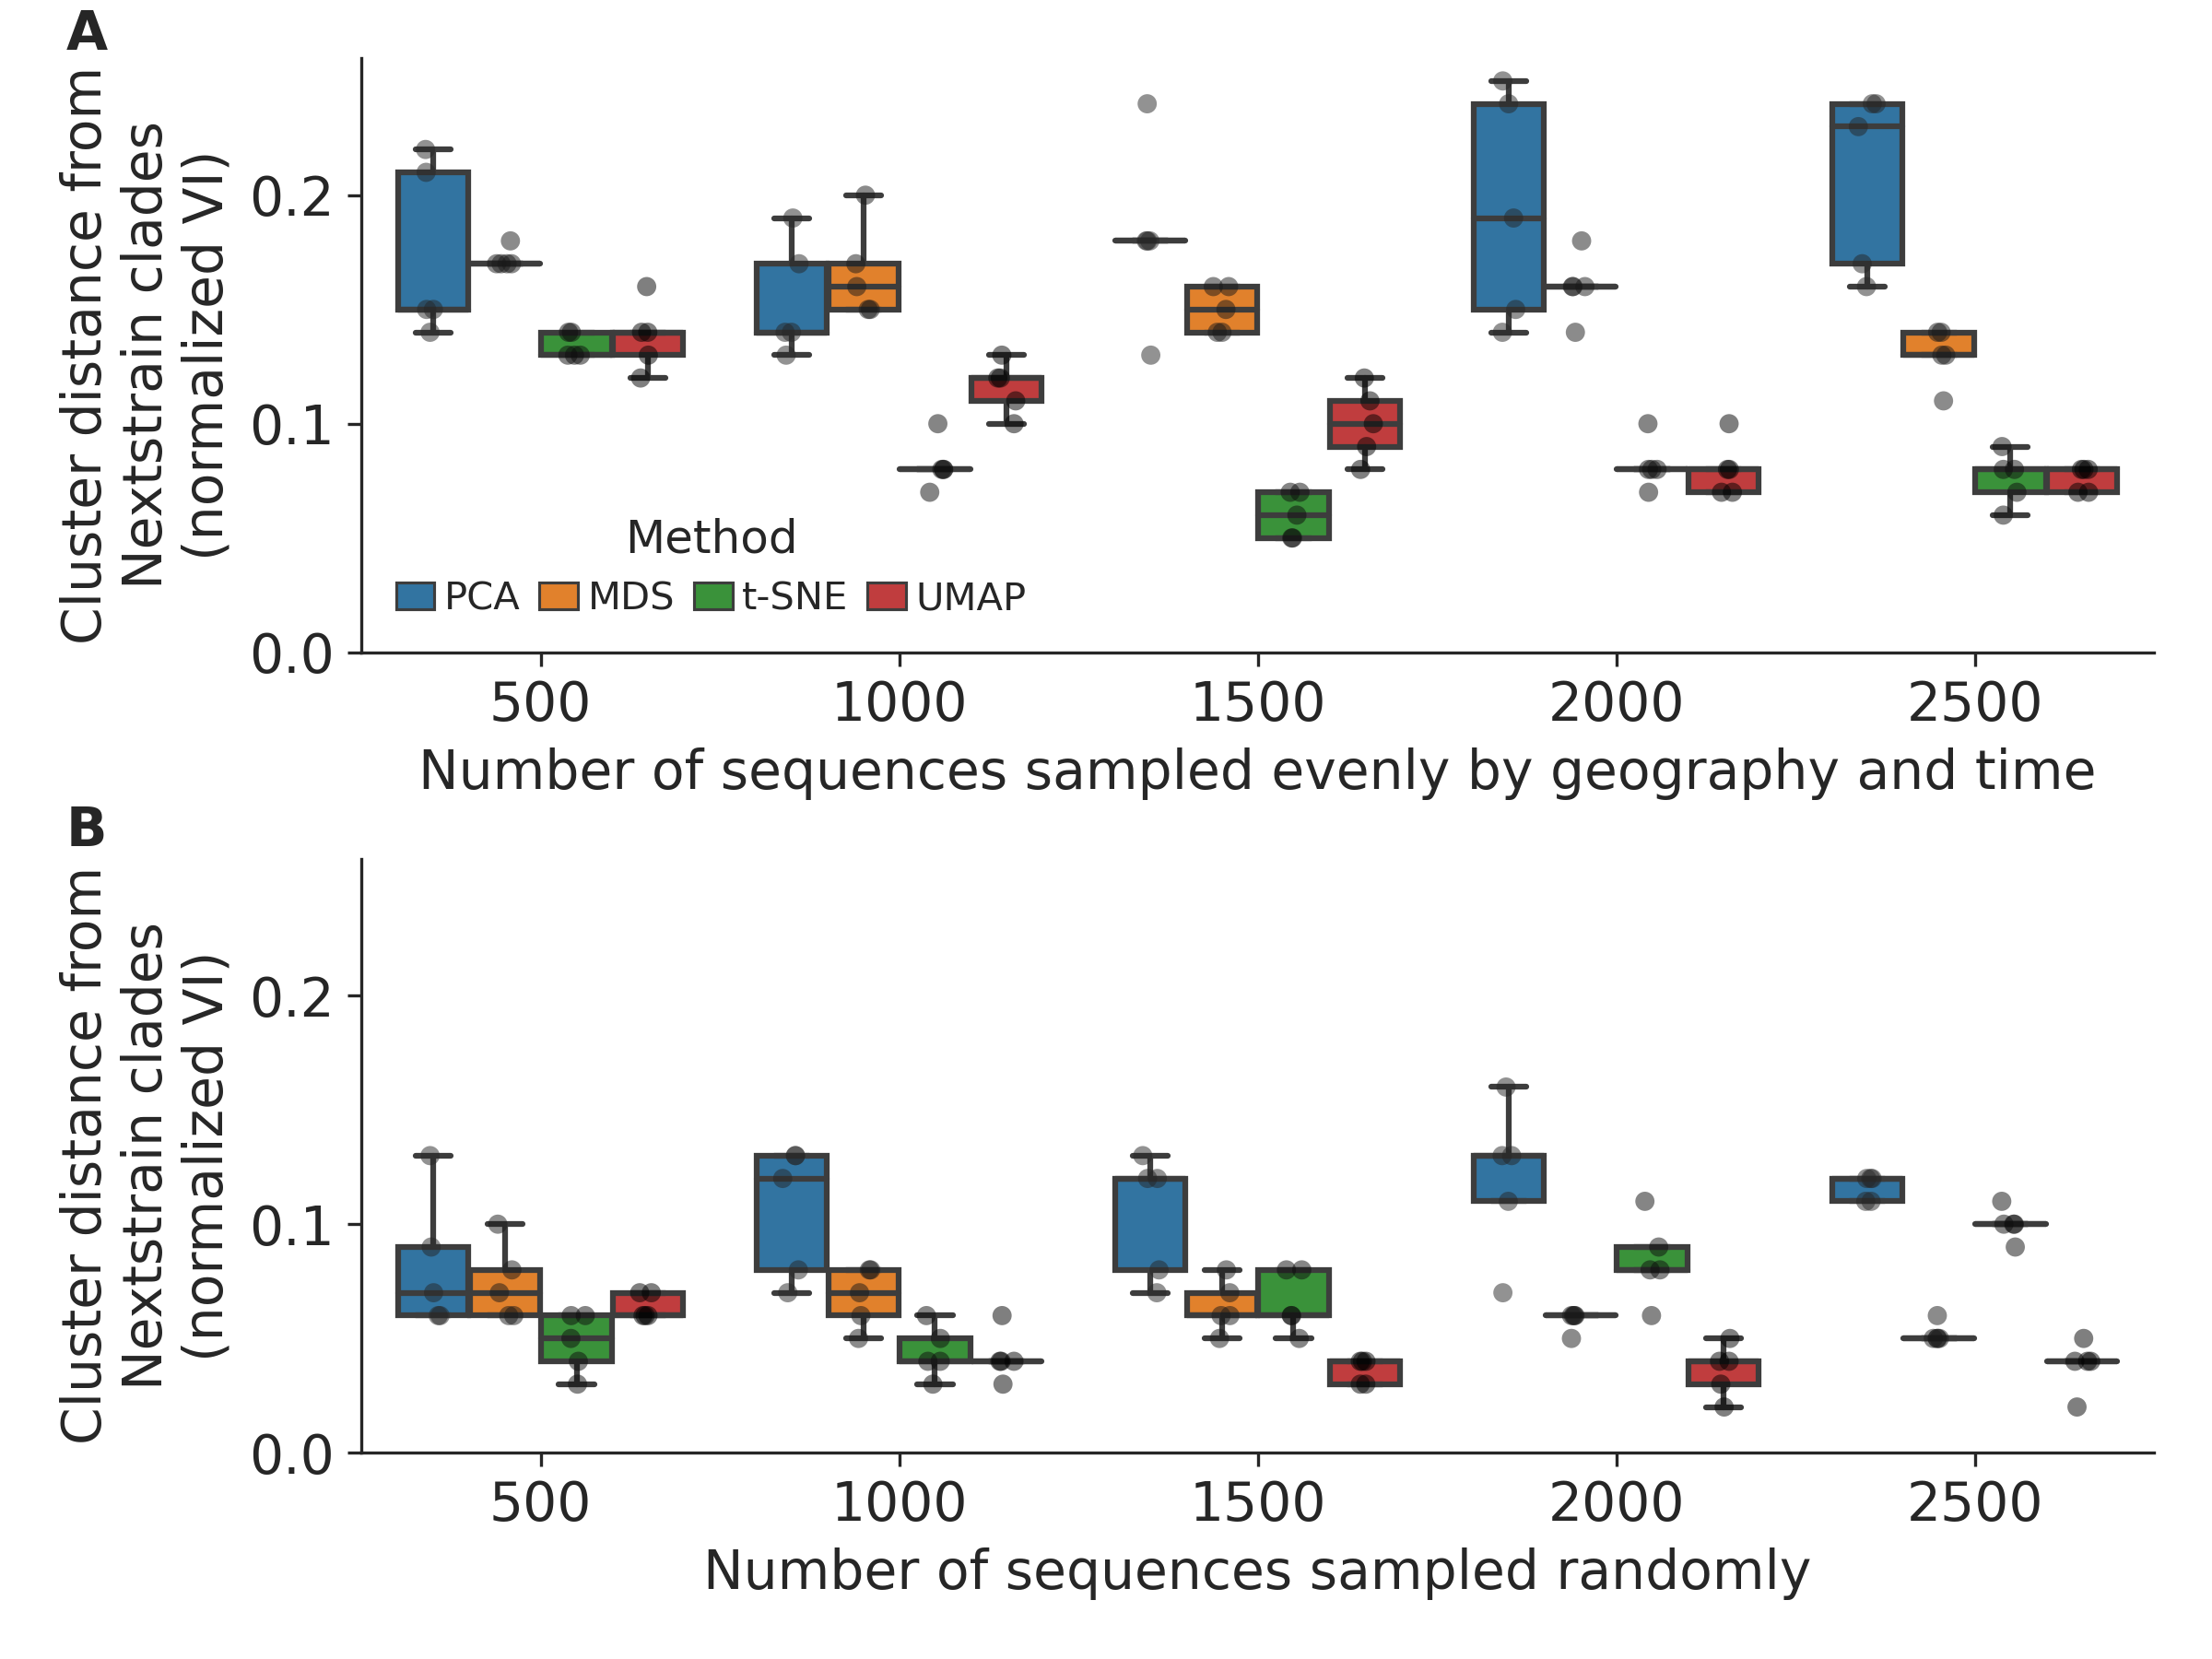
\includegraphics[width=\columnwidth]{figures/sarscov2-test-replication-of-cluster-accuracy.png}
\caption*{{\bf S18 Fig. Replication of cluster accuracy per embedding method for late (2022--2023) SARS-CoV-2 sequences across different sampling densities (total sequences sampled) and sampling schemes including A) even geographic and temporal sampling and B) random sampling.}
  We measured cluster accuracy across five replicates per sampling density and scheme with the normalized VI distance between clusters from a given embedding and Nextstrain clades for the same samples.
  The even sampling scheme selected sequences evenly across region, year, and month to minimize geographic and temporal bias.
  The random sampling scheme uniformly sampled from the original dataset, reflecting the geographic and genetic bias in those data.
}
\end{figure}

\begin{figure}[!h]
% TODO: remove includegraphics commands in final submission; figures must be uploaded separately from the manuscript.
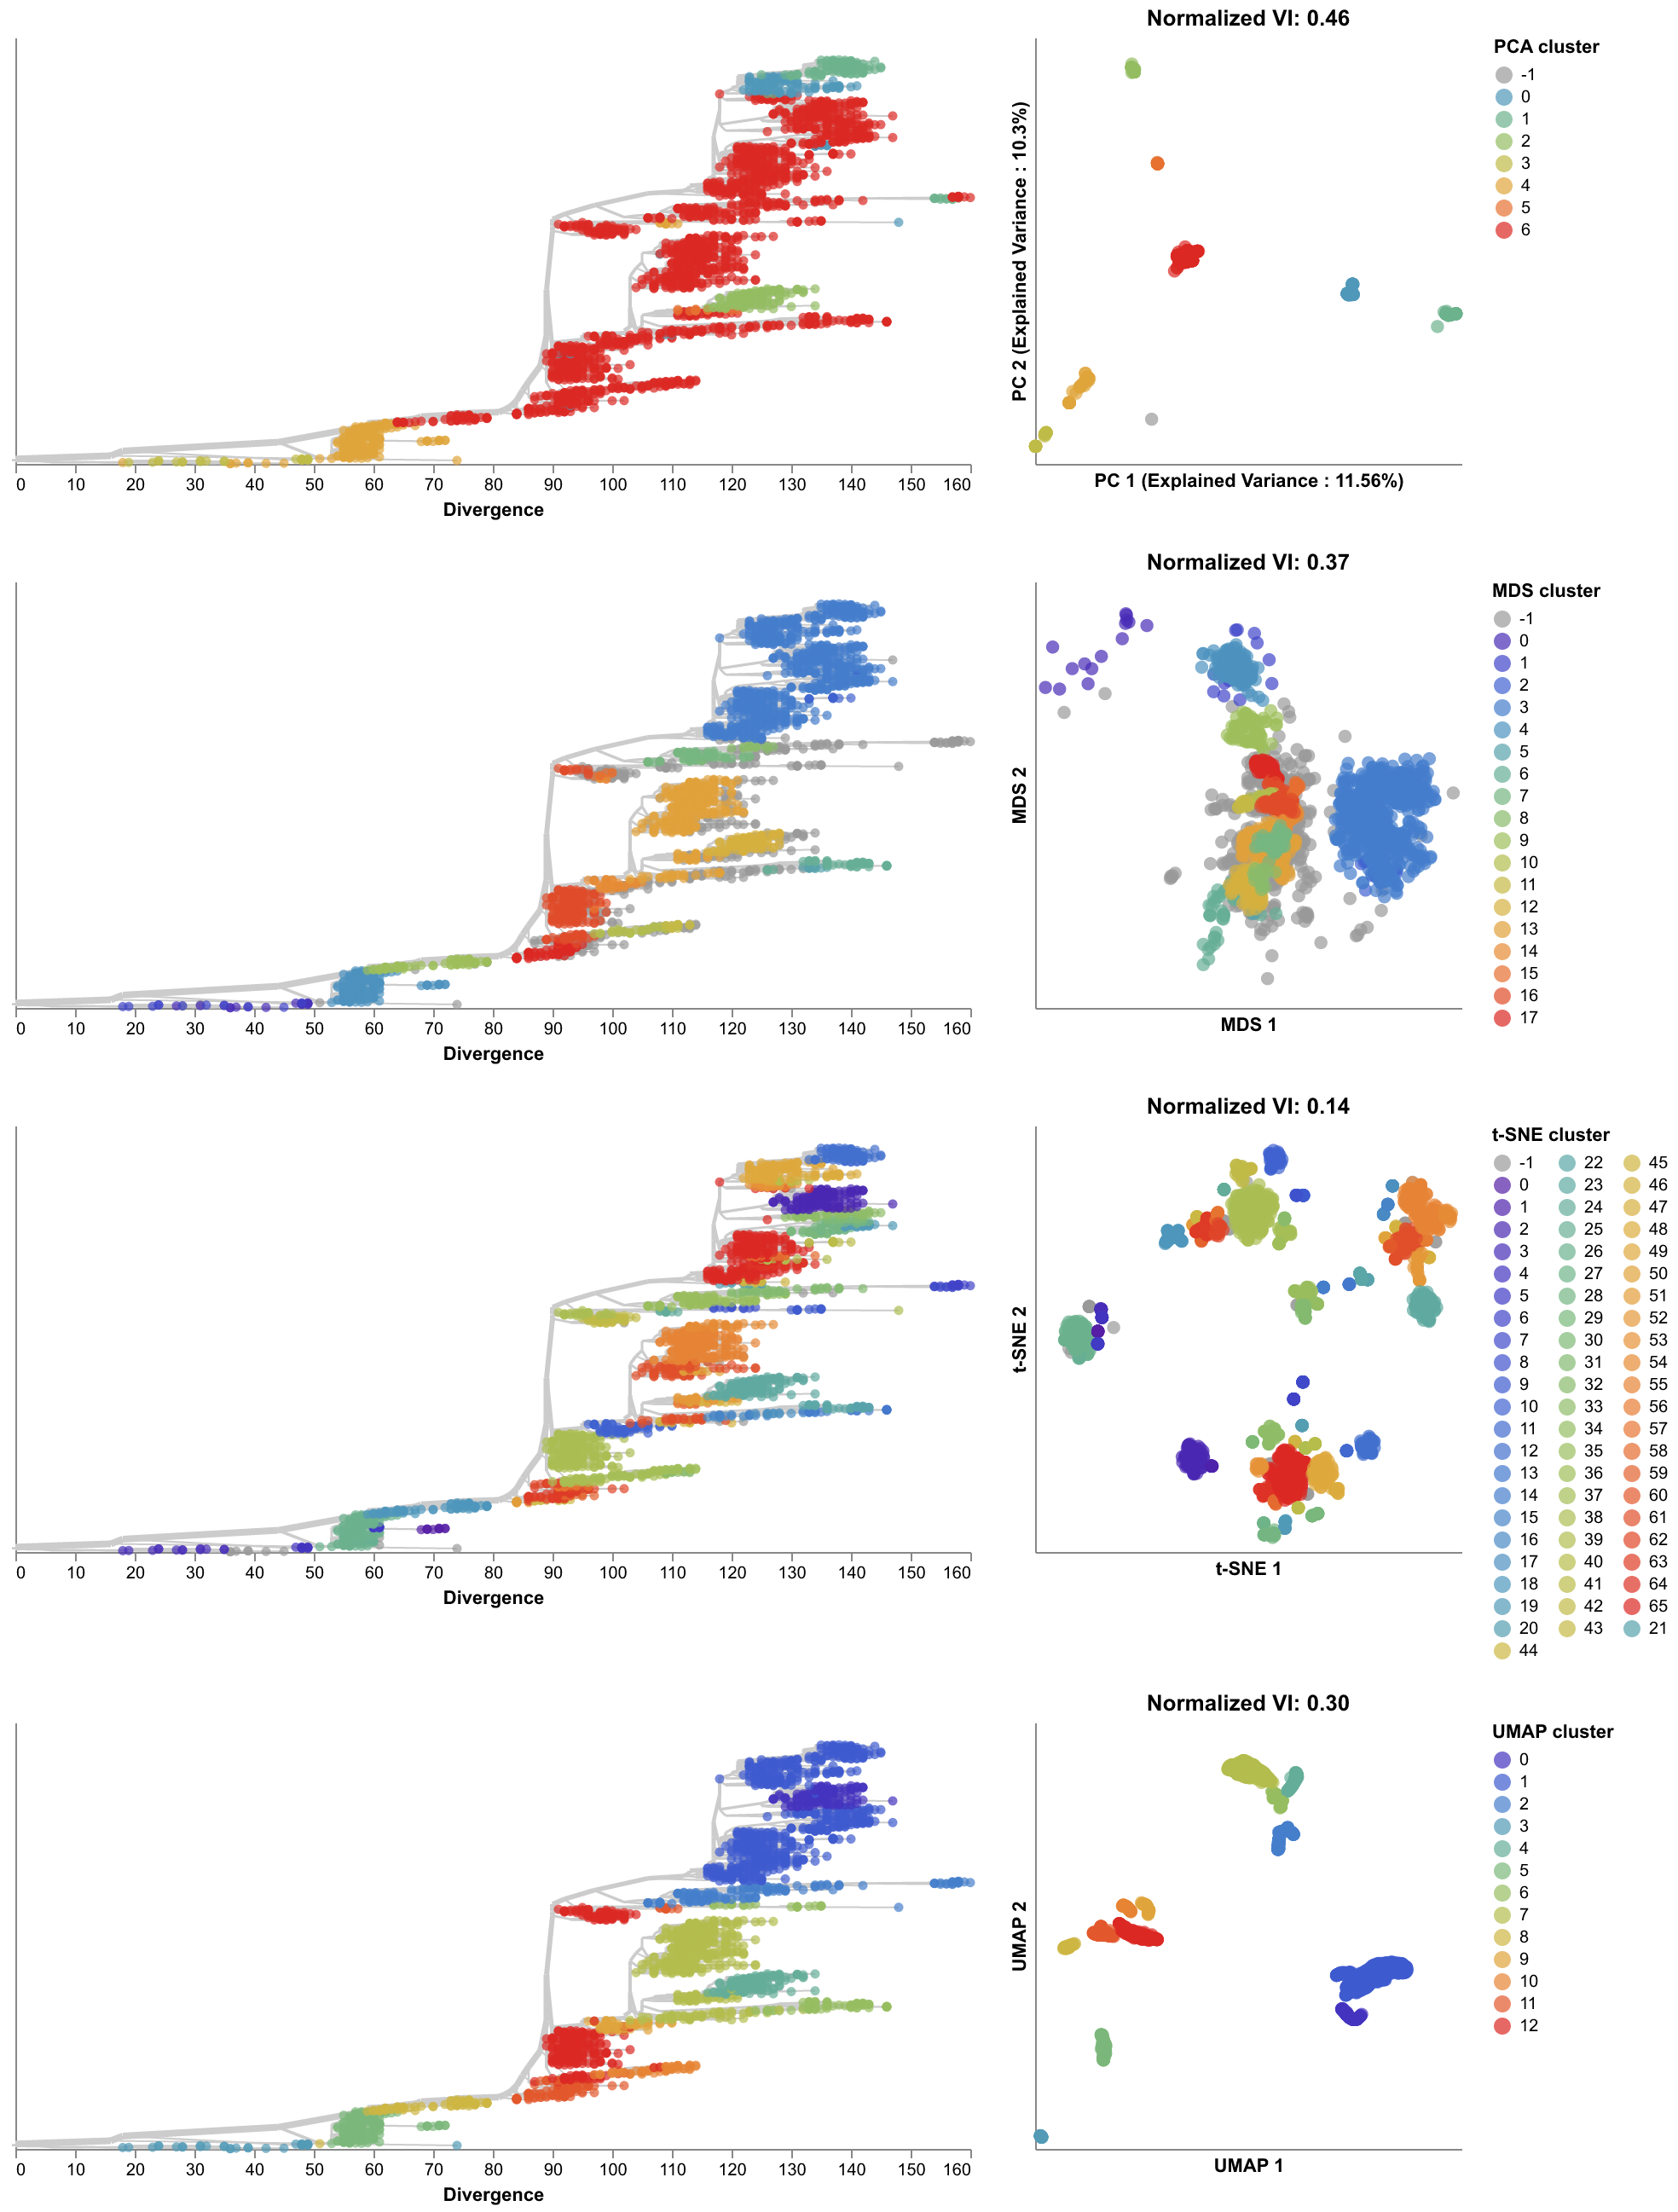
\includegraphics[width=\columnwidth]{figures/sarscov2-test-embeddings-by-cluster-vs-Nextclade_pango_collapsed.png}
\caption*{{\bf S19 Fig. Phylogenetic trees (left) and embeddings (right) of late (2022--2023) SARS-CoV-2 sequences colored by HDBSCAN cluster.}
  Normalized VI values per embedding reflect the distance between clusters and known genetic groups (Pango lineages).
}
\end{figure}

\nolinenumbers

% Either type in your references using
% \begin{thebibliography}{}
% \bibitem{}
% Text
% \end{thebibliography}
%
% or
%
% Compile your BiBTeX database using our plos2015.bst
% style file and paste the contents of your .bbl file
% here. See http://journals.plos.org/plosone/s/latex for
% step-by-step instructions.
%
% \begin{thebibliography}{10}

% \bibitem{bib1}
% Conant GC, Wolfe KH.
% \newblock {{T}urning a hobby into a job: how duplicated genes find new
%   functions}.
% \newblock Nat Rev Genet. 2008 Dec;9(12):938--950.

% \bibitem{bib2}
% Ohno S.
% \newblock Evolution by gene duplication.
% \newblock London: George Alien \& Unwin Ltd. Berlin, Heidelberg and New York:
%   Springer-Verlag.; 1970.

% \bibitem{bib3}
% Magwire MM, Bayer F, Webster CL, Cao C, Jiggins FM.
% \newblock {{S}uccessive increases in the resistance of {D}rosophila to viral
%   infection through a transposon insertion followed by a {D}uplication}.
% \newblock PLoS Genet. 2011 Oct;7(10):e1002337.

% \end{thebibliography}

\end{document}
